% The document class marks this as a thesis, supplying various options that

\documentclass[ % the name of the author
                    author={Sam Phippen},
                % the name of the supervisor (preferably including title)
                supervisor={Dr. Rafal Bogacz},
                % the thesis    title (which cannot be blank)
                     title={Real time voice activity detectors in noisy personal computing environments},
                % the thesis subtitle (which can    be blank)
                  subtitle={},
                % the degree programme (from BSc, MEng, MSci, MSc and PhD)
                    degree={MEng},
                % the year of submission
                      year={2012} ]{thesis}

\usepackage{parskip}
\usepackage{csvsimple}
\usepackage{rotating}


\begin{document}


% =============================================================================

% This section simply introduces the structural guidelines.  It can clearly
% be deleted (or commented out) if you use the file as a template for your
% own thesis: everything following it is in the correct order to use as is.

\section*{Prelude}
\thispagestyle{empty}

A typical thesis will be structured according to a number of standard 
sections described in what follows.  However, it is hard and perhaps
even counter-productive to generalise: the goal of outlining this 
typical structure is {\em not} to be prescriptive, but simply to act 
as a guideline.  In particular, the page counts given are important 
but not absolute: their aim is simply to highlight that a clear, 
concise description is better than a rambling alternative that 
makes it hard to separate important content and facts from trivia.

You can use this document as a \LaTeX-based~\cite{latexbook1,latexbook2}
template for your own thesis by simply deleting extraneous sections (e.g., 
this one); keep in mind that the associated {\tt Makefile} could be of
use, in particular since it also executes \mbox{\BibTeX} to deal with the
bibliography.  If you opt not to do this, which is perfectly acceptible,
a standard cover and declaration of authorship produced online via
\[
\mbox{\url{http://www.cs.bris.ac.uk/Teaching/Resources/cover.html}}
\]

% =============================================================================

% This macro creates the standard UoB title page, with information drawn
% from the document class (meaning it is vital you select the correct
% degree title and so on).

\maketitle

% After the title page (which is a special case in that it is not numbered)
% comes the front matter or preliminaries; this macro signals the start of
% such content, meaning the pages are numbered with Roman numerals.

\frontmatter

% This macro creates the standard UoB thesis declaration; on the hard-copy,
% this must be signed by the author in the space indicated.

\makedecl

% LaTeX will automatically generate a table of contents, and also associated 
% lists of figures, tables and algorithms.  The former is a compulsory part
% of the thesis, but if you do not require the latter they can be suppressed
% by simply commenting out the associated macro.

\tableofcontents
\listoffigures
\listoftables
\listofalgorithms
\lstlistoflistings

% The following sections are part of the front matter, but are not generated
% automatically by LaTeX; the use of \chapter* means they are not numbered.

% -----------------------------------------------------------------------------

\chapter*{Executive Summary}

{\bf A compulsory section, of at most $1$ page} 
\vspace{1cm} 

\noindent
This section should pr\'{e}cis the project context, aims and objectives 
and main contributions and achievements; the same section may be called
an abstract elsewhere.  The goal is to ensure the reader is clear about 
what the topic is, what you have done within this topic, {\em and} what 
your view of the outcome is.

The former aspects should be guided by your specification: essentially 
this section is a (very) short version of what is typically the first 
chapter.  The latter aspects should be presented as a concise, factual 
bullet point list that summarises the main contributions and achievements.  
The points will of course differ for each project, but an example is as 
follows:

\begin{quote}
\noindent
\begin{itemize}
\item I spent $120$ hours collecting material on and learning about the 
      Java garbage-collection sub-system. 
\item I wrote a total of $5000$ lines of source code, comprising a Linux 
      device driver for a robot (in C) and a GUI (in Java) that is 
      used to control it.
\item I designed a new algorithm for computing the non-linear mapping 
      from A-space to B-space using a genetic algorithm, see page $17$.
\item I implemented a version of the algorithm proposed by Jones and 
      Smith in [6], see page $12$, corrected a mistake in it, and 
      compared the results with several alternatives.
\end{itemize}
\end{quote}

% -----------------------------------------------------------------------------

\chapter*{Supporting Technologies}

{\bf A compulsory section, of at most $1$ page}
\vspace{1cm} 

\noindent
This section should present a detailed summary, in bullet point form, of 
any third-party resources (e.g., hardware and software components) used 
during the project.  Use of such resources is perfectly acceptable: the 
goal of this section is simply to be clear about where and how they are 
used.  The content can focus on the project topic itself (rather than, 
for example, including ``I used \mbox{\LaTeX} to prepare my thesis''); 
an example is as follows:

\begin{quote}
\noindent
\begin{itemize}
\item I used the Java {\tt BigInteger} class to support my implementation 
      of RSA.
\item I used a parts of the OpenCV computer vision library to capture 
      images from a camera, and for various standard operations (e.g., 
      threshold, edge detection).
\item I used an FPGA device supplied by the Department, and altered it 
      to support an open-source UART core obtained from 
      \url{http://opencores.org/}.
\item The web-interface component of my system was implemented by 
      extending the open-source WordPress software available from
      \url{http://wordpress.org/}.
\end{itemize}
\end{quote}

% -----------------------------------------------------------------------------

\chapter*{Notation and Acronyms}

{\bf An optional section, of roughly $1$ or $2$ pages}
\vspace{1cm} 

\noindent
Any well written document will introduce notation and acronyms before their 
use, {\em even if} they are standard in some way: this ensures any reader 
can understand the resulting self-contained content.  

Said introduction can exist within the thesis itself, wherever that is
appropriate.  For an acronym, this is typically achieved at the first point 
of use via ``Advanced Encryption Standard (AES)'' or similar, noting the 
capitalisation of relevant letters.  However, it can be useful to include 
an additional, dedicated list at the start of the thesis; the advantage of 
doing so is that you cannot mistakenly use an acronym, for example, 
before defining it.  An example is as follows:

\begin{quote}
\noindent
\begin{tabular}{lcl}
VAD                 &:     & Voice Activity Detection                 \\
VOIP                &:     & Voice Over IP\\
%DES                 &:     & Data Encryption Standard                \\
%                    &\vdots&                                         \\
%${\mathcal H}( x )$ &:     & the Hamming weight of $x$               \\
%${\mathbb  F}_q$    &:     & a finite field with $q$ elements        \\
%$x_i$               &:     & the $i$-th bit of some bit-sequence $x$ \\
\end{tabular}
\end{quote}

% -----------------------------------------------------------------------------

\chapter*{Acknowledgements}

\vspace{1cm}

This thesis would not have been possible without the continual support of my
supervisor {\bf Dr Rafal Bogacz}, who has spent many hours with me this year giving
me advice on how to organise the execution of this project, as well as ideas
for how to make improvments when I was stuck.

I would also like to thank:
\begin{itemize}

    \item My friend and mentor {\bf Dr Ben Fields}, who spent a couple of his
        afternoons discussing my thesis with me, and also for sharing his
        personal experience of writing 3 theses of his own.

    \item My good friends {\bf James Laverack} and {\bf Luke Murray} with whom I spent a
        huge amount of time unwinding when I felt burnt out.

    \item My {\bf parents}, who provided me with a much needed supply of tea during
        the long writeup of this thesis.

\end{itemize}

% =============================================================================

% After the front matter comes a number of chapters; under each chapter,
% sections, subsections and even subsubsections are permissible.  The
% pages in this part are numbered with Arabic numerals.  Note that:
%
% - A reference point can be marked using \label{XXX}, and then later
%   referred to via \ref{XXX}; for example Chapter\ref{chap:context}.
% - The chapters are presented here in one file; this can become hard
%   to manage.  An alternative is to save the content in seprate files
%   the use \input{XXX} to import it, which acts like the #include
%   directive in C.

\mainmatter

% -----------------------------------------------------------------------------

\chapter{Contextual Background}
\label{chap:context}

\vspace{1cm}

The term voice activity detection (sometimes referred to as voice endpoint
location\cite{Tuske}) refers to the algorithms used to distinguish frames of
audio that contain speech from those that contain background
noise\cite{ramirez}. The motivation for this project is that we found, based on
personal experience, that existing VAD algorithms struggle to efficiently
distinguish the noise commonly associated with personal computers (typing and
mouse clicks) from speech.

\section{Applications}

The two main applications of VAD systems are VOIP and Speech Recognition. These
systems both deal with human voice coming in from microphone input, and are
only concerned with what the people that are actually saying, rather than the
entirety of any particular audio sequence. Given these constraints it seems
natural to place a system which only passes through the parts of the audio that
contain human speech.

\subsection{Speech Recognition}

Speech recognition systems are responsible for working out what is being said
in a given sequence of audio. They must be robust to different speakers,
environments, hesitation, stuttering and other human factors. It is often noted
that these systems degrade rapidly in the presence of noise\cite{Moreno} given
that increasingly with systems like Siri\texttrademark\cite{siri} (Apple's
speech recognition system for iOS\texttrademark) we find that people are using
systems that require accurate detection of what is being said in potentially
noisy outdoor environments.

Speech recognition systems can have their accuracy improved\cite{shin} by
employing VAD systems, which are used to locate speech endpoints. The speech
endpoints are then passed into the speech recognition system which then has to
only search the places that the VAD system has flagged up for words, rather
than the entire sequence of audio. If the VAD system is sufficiently sensitive
it may also be able to accurately locate the pauses between words the user
makes, allowing the speech recognition system to assume 1 or very few words
will lie within each part of detected speech.

There is a well known speech recognition benchmark suite called
Aurora\cite{aurora}, over this benchmark suite it was found\cite{ramirez-2}
that by improving the VAD used from the G.729 ITU-T\cite{itut} standard to a
specialised detector that word accuracy (the number of words correctly
recognized) jumped approximately 17\% in the best case.

In the context of this project we believe that our detector may be able to
improve speech recognition through improved voice activity detection, but it is
not our primary goal, as we forsee fewer circumstances where a user is going to
require speech recognition whilst interacting with their computer, than we see
cases where VOIP calls are occurring at the same time as someone is interacting
with the keyboard and mouse inputs.

\clearpage
\subsection{VOIP and Telephony}

When used in a VOIP context VAD systems are typically designed such that they
signal that frames detected as noise are not to be transmitted, preventing the
person at the other end of the call from hearing the noise. Often this is a
component in a system that also includes some noise filtering and compression
the mumble\cite{mumble} system for example includes both an amplitude and
signal-noise ratio based VAD, and then passes the output into the
CELT\cite{celt} codec, here the VAD system silences any noise detected frames
and CELT efficiently compresses the silence to ensure a bandwidth saving.

VAD algorithms allow for large bandwidth savings during both analogue
telephone calls and VOIP calls. The reason for this bandwidth saving is that in
both dialogue (two people speaking) and monologue (one person speaking) much of
the time of the call is occupied by silence. Specifically: 60\% of the time is
occupied by neither person speaking\cite{shah} in a dialogue and 20\% of the
time is occupied by neither person speaking in a monologue.

In the case of a traditional analogue telephone call, the bandwidth saving is
achieved by "Time Assigned Speech Interpolation" whereby a link can carry more
calls by assigning resources only to those calls that currently have someone
speaking on them, causing a significant saving when, for example, speech is
only travelling in one direction (1 slot instead of 2) or allocating no slots
to the call when neither party is speaking\cite{5016247}.

With a VOIP call, a significant bandwidth saving is achieved by nature of the
fact that if transmission were continuous, both parties would be transmitting
at least 64,000 bits per second\cite{ciscovad}. If we assume that for most of
the call only one person is speaking, and that our VAD is sufficiently good at
distinguishing noise from human speech then we will find at least a 50\%
bandwidth saving. Additionally if there are pauses in speech, the VAD will
provide an even greater bandwidth saving.


\section{Problem Definition}

Seeing that both user experience can be improved, and that bandwidth savings
can be achieved through the use of voice activity detection systems, the
question is what can be done to improve these. The specific goal of this
project is to build a voice activity detection system which is robust in the
typical environment of a modern computer user. Whilst these environments do
have a low background noise, they often contain very high amplitude noise
impulses that are caused by the user typing on the keyboard, or interacting
with the mouse.

As is discussed in the implementation section of this project we show that
these systems do not have a high detection accuracy when presented with these
noise impulses. Our aim is to build a VAD system that does provide a high level
of accuracy against this specific type of noise.

We believe that the problem in modern systems exist because most VAD algorithms
are designed for noisy background environments\cite{shin}, but they are not
designed for short, loud noise impulses. These noise impulses are common when a
user is typing on their keyboard. There are two modern consumer VOIP systems
that we used and were found to detect keyboard noise or mouse noise as someone
speaking. Those were: Mumble\cite{mumble}, a low latency system designed for
gamers to communicate whilst playing with each other and
Skype\texttrademark\cite{skype} a well known consumer VOIP solution designed
for single or many person VOIP calls. Especially in the case of mumble it is
essential that keyboard noise is filtered out, as gamers tend to be interacting
with their keyboard continuously whilst playing videogames, possibly drowning
out much of the real communication, or causing annoyance.

The high-level objective of this project is to build a robust voice activity
detector system that can accurately distinguish voice from keyboard and mouse
noise with suitable performance for use in real time systems. More specifically
the concrete aims are:

\begin{enumerate}
    \item Survey existing VAD systems for accuracy against our dataset
    \item Work to develop own algorithm based on machine learning techniques,
          using common features from literature
    \item Build a hangover system which smooths transition from voice to 
          non-voice classes
\end{enumerate}



% -----------------------------------------------------------------------------

\chapter{Technical Background}
\label{chap:technical}

{\bf A compulsory chapter, of roughly $10$ to $20$ pages} 
\vspace{1cm} 

\noindent

%\section {danpagematter}
%This chapter is intended to describe the technical basis on which execution
%of the project depends.  The goal is to provide a detailed explanation of
%the specific problem at hand, and any previous or related work in the area 
%(e.g., descriptions of supporting technologies, existing algorithms that 
%you use, alternative solutions proposed).  
%
%Put another way, after reading this chapter a non-expert reader should have 
%obtained enough background to understand what {\em you} have done, and then
%assess how novel, challenging and rigorous your work is.  You might view an 
%additional goal as giving the reader confidence that you are able to absorb 
%and understand research-level material.

The basic problem any voice activity detector is trying to solve is the
question of whether or not a particular frame of audio does or does not contain
speech.

In nearly all recording environments there is continuous background
noise and, when there is speech, the microphone picks up speaking on top of
that. Thusly the output of a VAD system is a single bit (1 or 0 for voice or
noise). In a VAD system we take input from the microphone and then attempt to
determine which of two input classes we are in, corresponding to whether we
should or should not transmit the audio further. We formulate this as a
decision as follows:

\begin{figure}
\[ decision = \left\{ \begin{array}{ll}
            1 & \mbox{if input like $n + v$: speech present}\\
    0 & \mbox{if input like $n$: no speech present}.\end{array} \right. \]
            \label{eqn:decision 1}
            \caption{Decision model for most voice activity detectors}
        \end{figure}

Where $n$ represents the presence of background noise and $v$ represents the
presence of conversational speech. This is referred to as additive
noise\cite{sohn} and generally represents a very realistic model of most
environments in which human speech must be differentiated from background noise.

In this project our problem space is slightly different, in that not only do we
have to deal with background noise but we also have to deal with the fact that
keyboard noise is picked up by microphones. This noise is in no way constant:
whilst most people type with a rhythm there are distinct impulses and times
when the amplitude from this noise is very low. In addition to this we may have
to deal with the case where someone is typing and talking at the same time. This
means that our decision model may look something like:

\begin{figure}
\[ decision = \left\{ \begin{array}{ll}
            1 & \mbox{if input like $n + k + v$: speech present}\\
            0 & \mbox{if input like $n + k$: no speech present}\\
    \end{array} \right. \]
            \label{eqn:decision 1}
            \caption{Decision model for our voice activity detector}
\end{figure}

Where $k$ represents the keyboard noise component of the input. This problem is
different as mentioned above, due to the highly non-static nature of keyboard
noise. It is worth noting that this model is still entirely additive, this
model is reasonable because the sources of noise should not destructively
interfere with each other. It is, however, worth noting that the phenomenon of
clipping, the decibel level of the sound sources the microphone can pick up
adding to go above it's input limit, can occur and in this case the additive
models may break down in chapter \ref{chap:evaluation} we investigate
how important these effects are.

Nearly every existing voice activity detector makes the assumption that
background noise is continuous, if irregular in volume and frequency, and
attempts to distinguish voice from the background noise. More commonly than not
we have found that these detectors merely identify any sound that is not part
of the continuous background noise, giving real scope to our project.
Specifically identifying sudden impulses of sound from the background, and
determining whether or not they are someone speaking or someone typing is the
main aim of our system.

\section{Understanding voice}

In particular there are two types of speech, voiced and unvoiced speech. The
easiest way to demonstrate the difference between this is to place two fingers
on your throat/lower chin and then make a "sssssssss" sound (unvoiced) followed
by a "zzzzzzzzzzzz" sound (voiced). In the first example one cannot feel any
vibration, however in the second example one feels ones throat vibrating.
Voiced and unvoiced speech have somewhat different characteristics and this
must be taking account of when building a VAD system.

When speaking voice typically has it's fundamental frequency in the 75-150HZ
range for men and the 150-300HZ range for women. However, the human voice when
speaking also has a rich harmonic content meaning that there are a number of
other frequency peaks. The voice band, the band used for transmission of speech
lies in the 300HZ to 3400HZ range. Whilst this may seem that it would cut off
the sound of voice. This is not the case as enough of the harmonics of speech
still make it through, and the listener will get the impression that they are
actually hearing the missing fundamental tone.

The harmonics of the fundamental are integer multiples in frequency of the
original note, demonstrated by figure \ref{img:harmonics}, we see that the
first harmonic is the wave with a base frequency, the second is with twice that
frequency and so on. Due to the complex physics of how our bodies force air through
our throats we get a large frequency response not only at the fundamental notes
of voice, but also at the first few harmonics of the fundamental.

We can see that a section of voice features strong harmonics of the fundamental
in figure \ref{img:spectrogram} a spectrogram, showing the frequency strength
over time for a segment of speech. Specifically with the first word note the
strong fundamental at 600HZ with strong harmonics at 1800HZ (3rd harmonic) and
2400HZ (4th harmonic).

\begin{figure}
    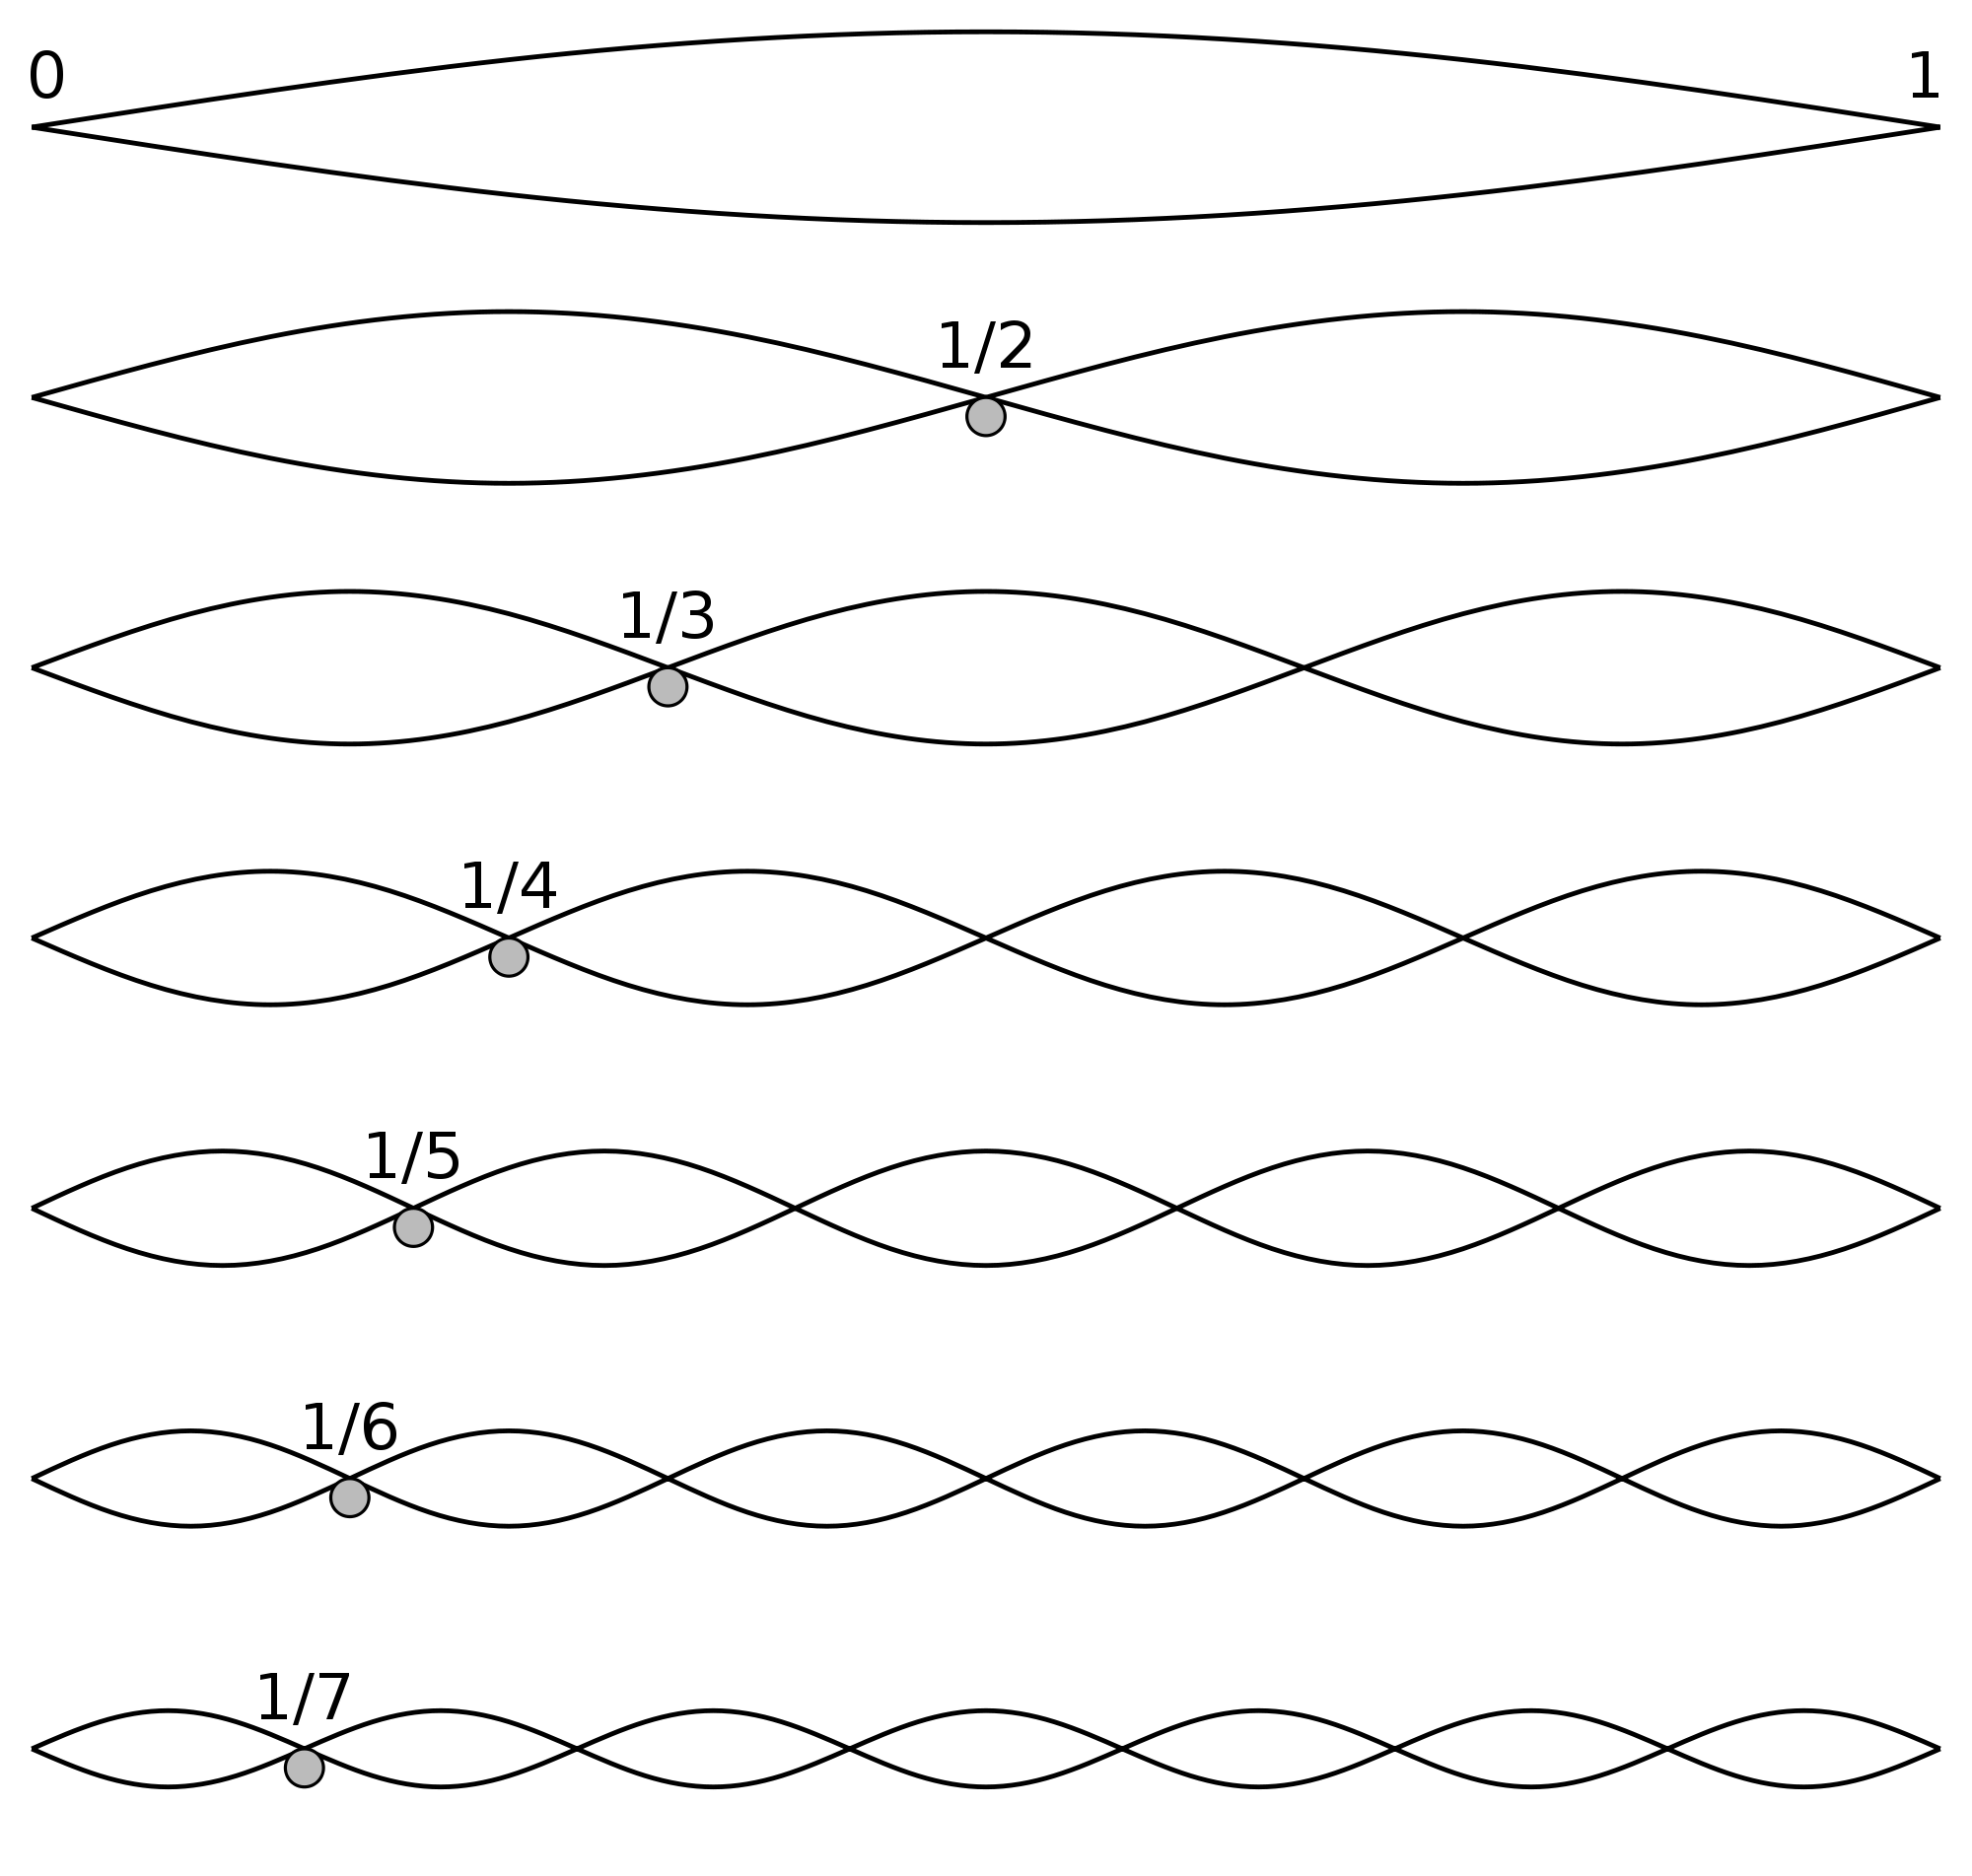
\includegraphics[height=10cm]{harmonics.png}
    \label{img:harmonics}
\end{figure}

\begin{figure}
    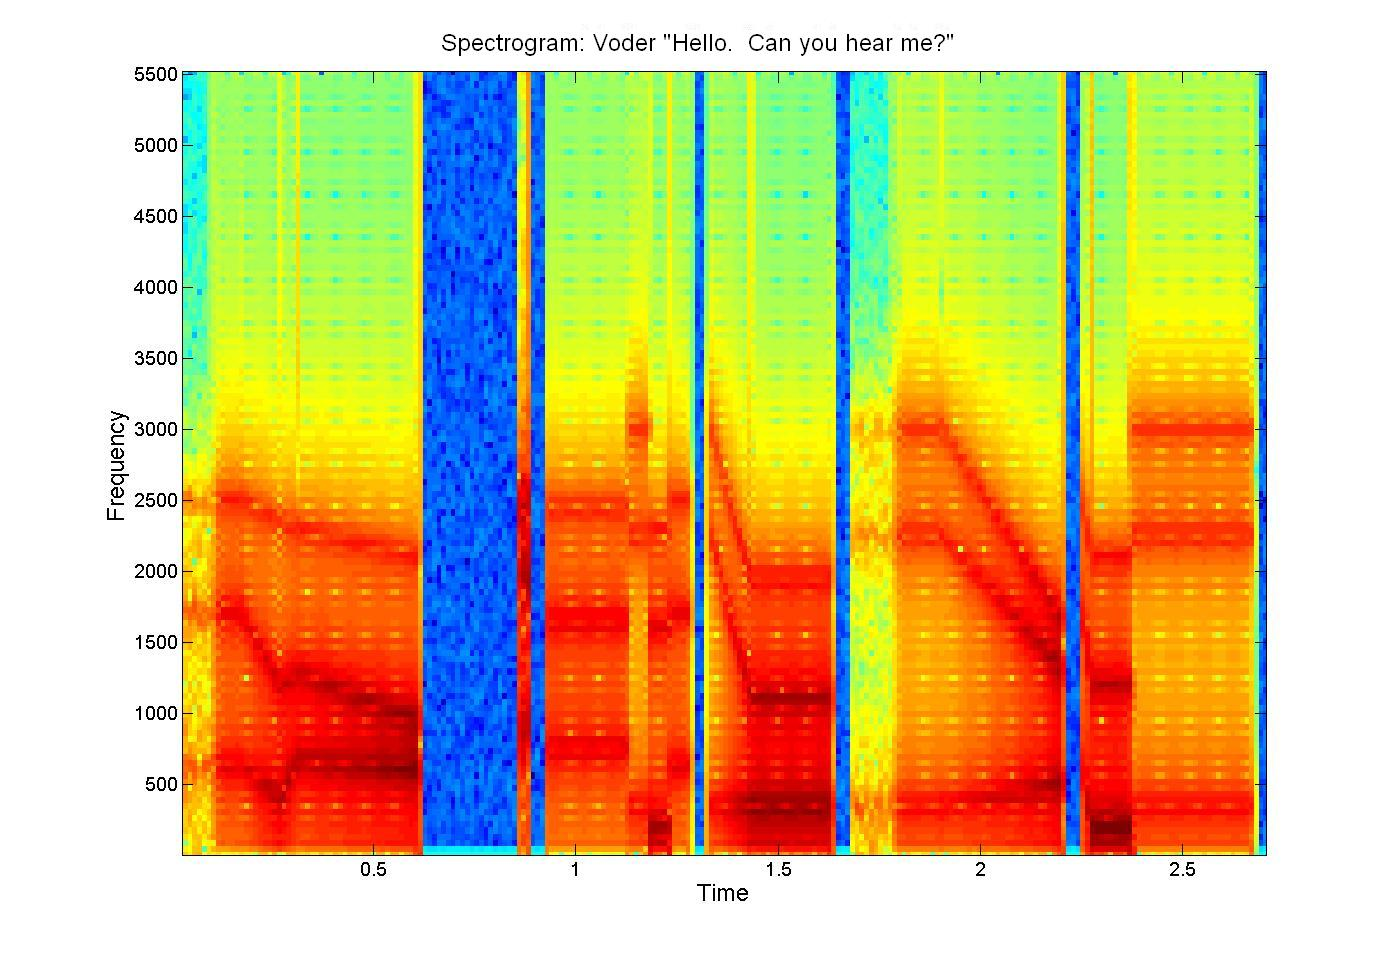
\includegraphics[height=10cm]{voder_spectrogram.jpg}
    \label{img:spectrogram}
\end{figure}

\section{Existing Voice Activity Detection Techniques}

Existing voice activity detection techniques fall into one of two categories.
Either the algorithms contain a number of parameters, and each parameter is
given a threshold (the noise/voice threshold). A decision is made based on the
thresholds over all the parameters as to whether transmission should or should
not occur. In some systems the thresholds are static with the thresholds
determined experimentally over some training data\cite{haigh}. These systems,
by their design have trouble dealing with background noise that changes such as
computer fans spinning up/down, or a person using a mobile phone walking through
streets with different activities happening in the background

In other threshold based voice activity detection systems the thresholds are
adaptive\cite{gokhun}. These systems are designed to deal with non-stationary
background noise, that is background noise that changes in amplitude and pitch.
These systems usually start with an initial guess of their class thresholds
which then change over time. The thresholds change based on the running average
of each of the parameter values for the two classes, as output by the
detector\cite{sakhnov}

The other major class of voice activity detectors apply machine learning
algorithms to build a complex classification boundary over the parameters of
the model\cite{shin}. These classifiers do suffer from the problem of having a static
decision boundary, due to the fact that on-line training is not possible
without hand labelling. This, however, usually does not cause too much of an
issue due to the fact that the more complex decision boundary achieves a much
higher accuracy when trying to decide between the voice and non-voice class.

\subsection {Features}

In both threshold based and machine learning based VAD systems a number of
features are extracted from the raw audio in order to give it a representation
that is amenable to distinguishing frames of audio that contain background
noise from those that contain speech. In this section we investigate existing
features that are used in models for voice activity detection, including those
that were and were not used in our model.

\subsubsection{Commonly used features}

When building our own classification system it is important to find the
features that are already being used to build VAD systems, such that they can
be used in our system, in combination with the classifier discussed in section
TODO ADD A REFERENCE SRSLY. Whilst our problem is slightly different in that we
have extremely non-stationary background noise, these features may be useful to
build an accurate VAD system. This also serves as the explanation for when
these features are referred to later on in this paper.

One of the most commonly used features in voice activity detection is the
energy of a frame. Given in figure \ref{eqn:energy} (sometimes also implemented
as the root mean square of a window), this feature is used in
\cite{shin}\cite{sakhnov}\cite{gokhun}\cite{haigh}\cite{atal} and \cite{sohn2}.
The energy feature of a particular window of audio has been found to be
significantly higher in frames that contain speech than background
noise\cite{atal}. However, this parameter also forms different distributions
for voice and unvoiced speech, with the energy value for voiced speech being
significantly higher than that for unvoiced speech. In \cite{atal} they state "
The energy of un-voiced sounds is usually lower than for voiced sounds, but
often higher than for silence." The system they used was a threshold based one,
however in \cite{shin} this feature was used as part of a decision tree system.
They reported "The full band energy, the conventional feature for endpoint
detection for clean speech, does not work well for noisy speech." The feature
did, however, give roughly 88\% accuracy figure by itself when used in their
classifier. This feature was used in our system for classification.

\begin{figure}
    $$Energy(x) = \sum_{i=0}^{length(x)}x(i)^2$$
    \label{eqn:energy}
    \caption{Energy of a window x, where length(x) gives the number of individual
    samples in x}
\end{figure}

Another commonly used feature in voice activity detection is the zero crossing
rate of a window. The definition for this feature is given in figure
\ref{eqn:zero-crossing-rate}. This feature is not used in \cite{shin}, but is
used in \cite{atal}. In \cite{atal} it is stated that zero crossing rate varies
consistently with energy. This is very important for a classifier based system
like the one that we are building because features that correlate with each
other weakly are likely to give different statistical "views" on the data that
machine learning algorithms can extract much of variance from in order to give
a more accurate classification. In \cite{shin} they state that zero-crossing
does not perform well in noisy speech, they did not use this parameter at all
and did not make any actual reports on the accuracy of the feature. In
\cite{haigh} they found that a detector based on energy and zero-crossing rate
only failed in noisy conditions. This feature was also used in our detector.

\begin{figure} $$ZeroCrossingRate(x) =
    \sum_{i=1}^{length(x)}abs(sign(x(i-1))-sign(x(i)))$$ \label{eqn:zero-crossing-rate}
    \caption{Energy of a window x, where length(x) gives the number of
    individual samples in x, abs is the absolute value of a number, and sign
gives the sign of the number 1, 0, or -1 for positive, zero or negative numbers
respectively} \end{figure}

\subsubsection{Other features from existing systems}

There are anumber of other features that were used in the system we built that
came from existing implementations of voice activity detection. We here explain
these features so that the reader is aware of how the feature values are
calculated.

Another feature that is used in \cite{shin} is referred to as a "band energy".
This simply takes the energy as specified in \ref{eqn:energy} but instead of
computing it over the entire window, it is taken over the amplitude component
of a fourier transform that has had a band pass applied to it, with the
frequency band specified. For example the 300-3700HZ band energy that Shin et
al refer to (which corresponds to the audible range of a telephone system) is
computed by taking the sum of squared amplitudes of the components of the
amplitude domain of a fourier transform that lie within the 300-3700HZ
frequency range. In our system we used multiple band energies as discussed in
chapter \ref{chap:execution}.

In \cite{haigh} they used ceptral features for voice activity detection. There
are multiple transforms that are referred to as the "cepstrum" of a signal,
specifically the complex cepstrum, the power cepstrum and the phase
cepstrum\cite{childers}. The power cepstrum is defined in
\ref{eqn:power-cepstrum}. This feature is primarily used in speech recongition,
the higher order task of determining what words are being said, rather than
voice detection\cite{muda} and in \cite{atal} they criticize this approach for
VAD, stating that this feature requires a very high degree of periodicity
(singal approximately repeats itself with a fixed period) to provided an
accurate classification.

\begin{figure}
    $PowerCepstrum(f)=\mathcal{F}^{-1}\{\mbox{log}(\mathcal{F}\{ f(t) \}|^2)\}|^2$
    \caption{Definition of a power cepstrum. $f$ is our
    signal function, $\mathcal{F}$ is the fourier transform function. $|a|$}
    \label{eqn:power-cepstrum}

\end{figure}

Specifically in \cite{haigh} they use a cepstral distance measure defined as
the euclidian distance of the power cepstrums between the data they were
attempting to classify and a pre-defined 'code-book' of samples, selecting the
class of whichever example in the 'code-book' had the lowest euclidian
distance. This is equivalent to a single nearest neighbor classification. An
accuracy figure is not given however they were able to design the threshold of
their system such that it tripped at a very low voice likelyhood ratio (0.01) with
relatively low error.

In \cite{moattar} one of the key features that they extracted was the dominant
frequency component of the signal. This corresponds to the highest peak in the
fourier transform of the signal and is defined in \ref{eqn:dom-freq}. The
authors of the paper observed that this feature was helpful in discriminating
speech and silence frames. We observed problems with this feature due to the
nature of our windowing system which are discussed in \ref{chap:execution}. The
accuracy of this feature is reported in \cite{moattar} to have a greater than
80\% accuracy under even noisy conditions. However the caveat to this feature
for our project does apply that our noise is highly irregular and most
definitely not of stationary amplitude.

\begin{figure}
    $DominantComponent(f) = argmax_i(|\mathcal{F}(f(t))|)$
    \caption{Definition of the dominant component of a signal. $f$ is the singal
        function, $\mathcal{F}$ is the fourier transform. $argmax$ gives us the
        input corresponding to the maximum output of a function.}
    \label{eqn:dom-freq}
\end{figure}

In \cite{atal} they used two features constructed via a linear predictive
coding (LPC) analysis. The basic principle of linear predictive coding is that
the current sample can be approximated as a linear combination of the previous
samples\cite{rabiner}, the coding is the coefficients ($a_1,a_2,...,a_p$) that
each of the previous samples are combined with to give the prediction of the
coding. In \cite{atal} they specifically used a size 12 linear combination,
which means that each sample was predicted as a linear combination of the
previous twelve. It is important to note here that over short periods of
10-30ms voice signals are roughly periodic, and that it is obvious that $s(n)
\approx s(n-N_p)$ where $N_p$ is the length of the period. LPC techniques work
with window sizes that are significantly smaller than the period and still
accurately reconstruct the next part of the signal. The result of the LPC is a
number of coefficients that can be used to attempt to reconstruct parts of the
signal, however, they can also be used as parameters to both threshold and
classifier based systems. In \cite{atal} they used two parameters from the LPC:

\begin{itemize}

    \item The first coefficient of a 12 coefficient LPC analysis: this is the
        primary coefficient $a_1$ of the LPC analysis, corresponding to the
        sample nearest to the sample we are trying to predict.

    \item The energy of the error in the prediction made by the LPC. This is
        essentially defined as the error signal (computed by subtracting the
        signal predicted by the LPC and the actual signal). Energy is defined
        above as the sum of the squares of the signal in \ref{eqn:energy}. In
        the paper they state that this feature is equivalent to the ratio of
        the geometric mean of the spectrum to the arithmetic mean of the
        spectrum.  This makes it equivalent to the spectral flatness measure
        defined in \cite{moattar}

\end{itemize}

\section{Machine learning techniques}

In this project we decided to use machine learning techniques to build our VAD
system. This is primarily due to the fact that threshold based approaches
report lower accuracy rates in the literature and are very much designed to
differentiate continuous background noise from sudden changes in any of their
parameters. Our feeling was that this would not be amenable to differentiating
sudden keyboard impulses from sudden voice impulses. In the execution chapter
of this project we discuss how we built the training set and how we built the
training set for this system, and this section specifically conducts a review
of machine learning systems, with an explanation of state of the art machine
learning techniques such as random forests, gradient boosted regression trees
and adaboost with decision stumps. All classifiers here are discussed under the
assumption that they only have to deal with a binary classification problem,
which corresponds to the classification problem that we are dealing with
(voice/non-voice classification).

\begin{figure}
    $Train:R^x \times R^y, \{0,1\}^y \rightarrow ModelFunction$

    \caption{Definition of a training function: x is the number of features and
        y is the number of classes. The function takes an x by y matrix of
        reals and a y-length vector of labels and ouptuts a model function that
        behaves as a classification function defined in in
    \ref{eqn:define-classify} }

    \label{eqn:define-train}
\end{figure}

\begin{figure}
    $Classify: R^x \rightarrow \{0,1\}$
    \caption{Definition of a trained model/classification function: x is the
        number of features, the model takes a feature vector and outputs a class,
    in some implementations this may be a probability}
    \label{eqn:define-classify}
\end{figure}

\subsection{Classification and regression trees}

Classification and regression trees are class of machine learning algorithm
that work by first training a binary decision tree and then pushing examples to
be classified through the binary decision tree to perform
classification/regression. Training is performed by computing splits in the
feature space that represent the maximum gain in information over the entire
set of features for the examples that will reach this part of the tree. At the
start the split that gives highest information gain over the entire data set is
chosen, giving us two subsets of the entire data set, that are then split
seperately from each other and so on and so on. This process continues until
the leaf nodes of the tree contain only training examples of the same class. By
this method we ensure that all training examples will be classified correctly,
in general this method can lead to some overfitting that will cause the classifier
to not generalise as well, and the trees are pruned. An example decision tree
is shown in Figure \ref{fig:decision-tree}.

\begin{figure}

    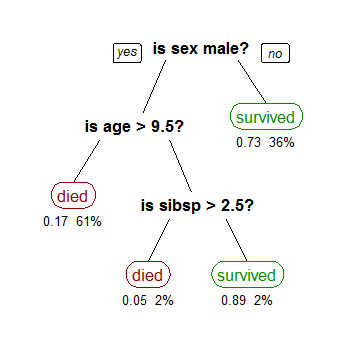
\includegraphics[height=10cm]{decision_tree.png}

    \label{fig:decision-tree}
    \caption{An example decision tree kindly provided by Wikipedia}
\end{figure}

Regression trees are used when the output is not a single class but instead
some single real number. For example a regression tree might be used in an
attempt to predict the length of a patients stay in hospital. In \cite{shin}
individual features were passed through a speech/non-speech classification, and
then a CART (classification and regression tree) was employed over the outputs
of the pre-classifiers to come to the final decision. This approach gave a very
high accuracy level under low and medium noise levels (-5 and 0db respectively)
but degraded under high noise levels (5db). In order to improve the
classification parmeters were passed in from more than one window (specifically
the previous and next window were passed in before the decision was made).

\subsection{Decision Stump}

Whilst never used on its own the decision stump classifier is worth exploring
due to it's use in ensemble\footnote{Ensemble classification methods are a
    large class of classification algorithm that combine many classifiers in an
    attempt to improve classification accuracy or generalizability or both. In
chapter \ref{chap:evaluation} we show that these methods give much better
accuracy in cross validation than non-ensemble techniques over our data set
with some intuition for why this is the case.} classification methods.
Specifically the decision stump classifier acts like a normal binary decision
tree classifier or CART but instead of training until completion it is trained
for only one split. These often acheive very low classifcation accuracy
(usually just barely better than a random classifier) and are sometimes
referred to as "weak" or "base" classifiers. In the famous Viola Jones face
detector\cite{viola} many decision stumps were used to form a strong classifier
that achieves very good classification accuracy. An example decision stump is
shown in Figure \ref{fig:decision-stump}.

\begin{figure}

    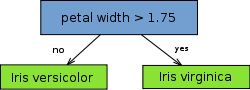
\includegraphics[width=5cm]{decision_stump.png}

    \label{fig:decision-stump}
    \caption{An example decision stump kindly provided by Wikipedia}
\end{figure}

\subsection{Adaboost}

Adaboost is a well known algorithm for ensemble classification that achieves
a high classification accuracy by training many classifiers. Unlike some of
the other ensemble methods we discuss in this paper the Adaboost method can
be used with any base classifier, and as such may be amenable to a larger set
of problems than other ensemble methods presented here. Specifically the result
of the Adaboost training is a chain of classifiers which become increasingly
biased towards the most difficult samples to accurately classify within the
training set.

The final classification output of the Adaboost algorithm is given as a linear
combination of weights multiplied by the classification output (usually a
posterior probability) of each of the individual classifiers within the Adaboost
classifier. The pseudocode for training the system is given in \ref{pseudo:adaboost}.

Within this paper we use an Adaboost algorithm that uses decision stumps as its
base classifier, this decision was made based on the fact that we wanted
training to complete quickly (decision stumps train in effectively no time) and
that this approach has been shown to work well in other problem
domains\cite{viola}.

It is worth noting that training an Adaboost classifier with a very large
number of weak classifiers can cause a high level of overfitting, especially
in the presence of noise within the data set.

\begin{figure}
    Psuedocode for training an adaboost classification system. It is important
    to note that the weak classifiers must be sensitive to the weights given in
    the $w$ array. If the classification system that is used is not sensitive
    to these weights (for example a decision tree by default has no concept of
    weighting it's inputs) we can weight the samples by performing a roulette
    wheel selection\footnotemark on the samples.

    \vspace{3em}

    \begin{enumerate}

        \item let $w_1(i)=\frac{1}{N_{samples}}$ for all $i$ in
            $0,1,...,N_{samples}$.

        \item for i = 0 to number of classifiers in ensemble (n)
            \begin{enumerate}

                \item Train a weak classifier that returns -1 or 1 given a
                    sample.
                \item Choose $\alpha_i \in R$.
                \item Update $w(i) = w(i)exp(-\alpha y_i h_t(x_i))$ for all $i$ in
            $0,1,...,N_{samples}$.
            \item Normalize $w(i)$ so that it sums to 1 (forms a probability distribution).

            \end{enumerate}
        \item output strong classifier: $$H(x) = sign\left(\sum_{i=0}^{n}\alpha_i h_i(x)\right)$$
    \end{enumerate}

    \vspace{3em}

    In step 2a in the previous listing we specifically pick the weak classifier
    that gives the lowest weighted prediction error over all the samples, where
    the weighted prediction error is defined as: $$error_{h_i} =
    \sum_{k=0}^{N_{samples}} w(k)(y_k\neq h_i(x_k))$$. By doing this at each
    stage we are effectively picking the weak classifier that is most capable
    of dealing with the most highly weighted samples. This gives us an improved
    classification over a single classifier because the difficult samples are
    given "specialist" classifiers that are more capable of dealing with them
    than a classifier trained over the entire set.

    In step 2b we specifically chose $\alpha_i$ to greedily minimize
    classification error at each step, that is at every step the overall
    classification error on the training set will go down rather than up.

    \label{pseudo:adaboost}
    \caption{Adaboost training psuedocode and explanation}

\end{figure}
\footnotetext{Roulette wheel selection is an algorithm which
        allows us to select randomly from a weighted array. If the array forms
        a probability distribution (that is that it sums to 1) then we can
        generate a number uniformly at random and move through the array of
        weights, subtracting each weight from the generated number, when the
        number reaches zero we have arrived at the item that corresponds to the
    randomly generated number, and we can output it. When performing this
selection multiple times we end up with a distribution of selections from the
array that matches the weights of the items.}

\subsection{Random Forest}
\label{section:random-forest}

The random forest classification algorithm is a modern ensemble method for
classification proposed by Breiman in \cite{breiman}. In a random forest many
decision trees are combined to give a much better classification result than
any single classifier is able to. In order to arrive at a final class the
original Breiman paper suggested that each classifier's output is taken and the
modal class is used. In the implementation that we use in this paper we instead
ask each tree to give a probability value that the instance is in the positive
(voice) class and then take the mean average of these, thresholding at 0.5 to
give the voiced/unvoiced classification. This helps to more accurately reflect
that some trees may be very confident with an instance and give a high
posterior probability but some may be less confident and give a probability
closer to 0.5, the mean of these allows the end result of the classification to
be more sensitive to the results of the individual trees.

The training method for a randomised forest as described in \cite{breiman} is
to create a randomised vector from the training set by performing selection
without replacement at random from the training set, such that any single
instance may occur more than once, this is the same technique that is used in
the bagging ensemble classification method. The difference between how this
system is trained, and how bagging trains is that instead of then just training
decision trees in the traditional way, the random forest approach builds splits
in each tree by selecting random subsets of the possible features at each of
the splits.

There is a second class of random forest used in this paper called extremely
randomised trees. This method goes one step further in the randomness during
training and instead of splitting on the most discriminative threshold of the
most discriminative feature of a random subset of the features at each training
stage the extremely randomised forest picks random thresholds of each feature
in the random subset of features and then picks the one with the highest information
gain.

In \ref{fig:comparison} we can see a comparison of decision trees, random forests,
extremely randomised trees and Adaboost. It is worth noting that the decision
boundaries for random forests are a lot noisier around noisy data than the
other classification algorithms.

\begin{figure} \label{fig:comparison}
    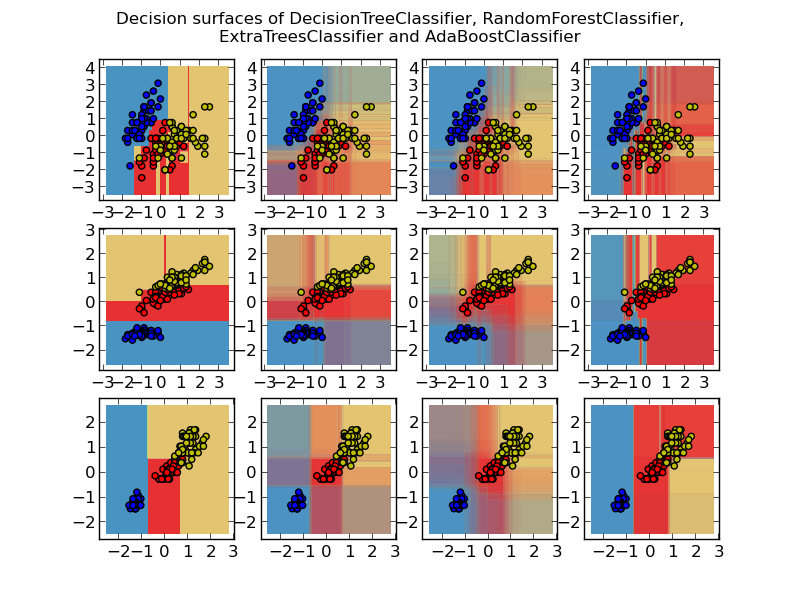
\includegraphics[width=13cm]{classifier_comparison.png} \caption{Comparison
        of decision trees and some ensemble classification techniques, showing
        data points with circles and decision boundaries with background color,
        shading in the background colour indicates probability where the
        ensemble methods have internal classifiers that disagree. The decision
        tree always has block color as it gives a single class as an output
rather than a probability} \end{figure}

\subsection{Gradient Boosted Regression Trees}

The gradient boosted regression trees algorithm uses boosting to build a strong
classifier by combining many decision trees over the input training samples.
Like Adaboost the GBRT (Gradient Boosted Regression Trees) model takes the
output of the overall classifier as the sum of each of the outputs of the
individual classifiers in the ensemble multiplied by a weight. The difference
between this technique and Adaboost is that instead of weighting samples that
are classified incorrectly, each internal classifier is trained with the
individual examples labelled with the residual between the actual label and
what the current version of the classifier gives.

The main disadvantage of GBRT in comparison to the Random Forest technique is
that the training process cannot be easily parallelized, due to the fact that
each new tree must be trained as a function of the ensemble classifier as it
has been trained thus far.

In \cite{parker} they use GBRT to perform sequence alignment of music, this
technique was also used by the winning submission to the netflix prize.

\subsection{A review of ensemble techniques}

The ensemble techniques that we have discussed sofar all have been shown to
perform significantly better in generic machine learning applications than
single classifiers this is because they build a number of different models in
various ways, each of which has either a randomised component, or is reliant on
moving against the error of other models within the ensemble. These techniques,
do, however come with a high performance overhead, due to the fact that there
are many classifiers instead of one. Adaboost with decision stumps does
somewhat serve as an exception to this rule because decision stumps take
virtually no time to perform a classification. In this paper we consider
decision trees, random forests, gradient boosted regression trees and Adaboost,
comparing the feature set that we developed in an attempt to maximise accuracy
and generalizability.

\section{ROC Curves}

A ROC curve, or Receiver Operating Characteristic curve, is a curve that is
used for evaluating the accuracy of a classifier by comparing the false
positive and true positive rate. The area under the ROC curve can also be used
as a measure of the accuracy of the classifier. In a 2 class problem, a
completely random classifier will strike a line of tpr = fpr at all points.
This is because it makes no decision. Better classifiers tend to move towards
better true positive rates and lower false positive rates, meaning that they
typically occupy the upper left half of the ROC curve. An example of this can
be seen in \ref{fig:roc-example}.

Note how several thresholds are pointed out on the curve. The reason for this
is that most classifiers do not output a binary class decision, but rather a
posterior probability or some other likelyhood that the example belongs to a
specific class. By thresholding the decision boundary, we can affect both the
true positive and false positive rate: this is particularly important in
classifiers that aren't merely going for raw maximum classification accuracy,
but rather care about a decision one way or the other. For example in our
classification problem it would be disasterous if some voice were not
transmitted when the user was speaking, so our system will naturally fall to
the lax threshold rather than the strict threshold.

\begin{figure}
    \label{fig:roc-example}
    \begin{center}
        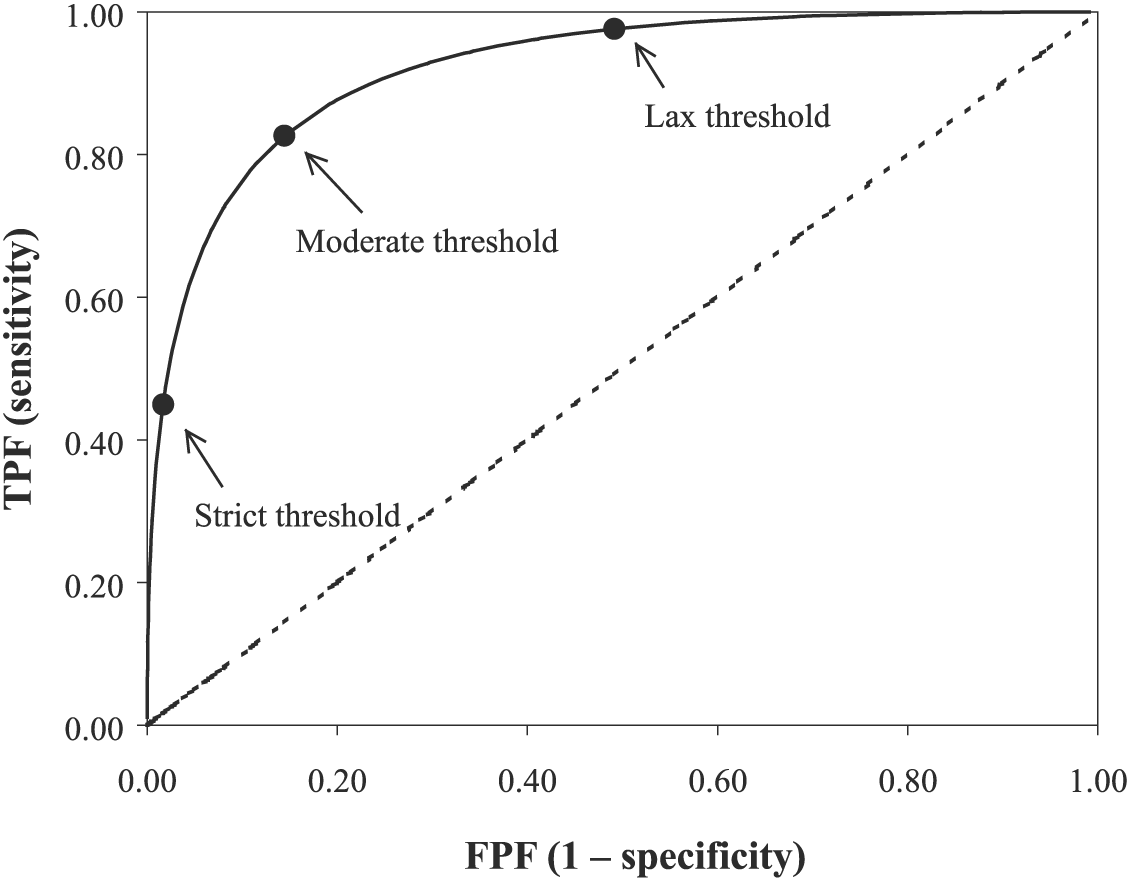
\includegraphics[height=10cm]{roc_example.png}
    \end{center}
\end{figure}

The area under the ROC curve is a measure of the predictive power of the
classifier\cite{fawcett}. No classifier used in the real world will have an
area under the ROC curve of less than 0.5, as random guessing will always
produce a diagonal line between (0,0) and (1,1). The specific meaning of the
AUC (area under the curve) statistic is, that it is the probability that the
classifier will rank a randomly chosen positive example more highly than a
randomly chosen negative example.

% -----------------------------------------------------------------------------

\chapter{Project Execution}
\label{chap:execution}

{\bf A topic-specific chapter, of roughly $20$ pages} 
\vspace{1cm} 

%\noindent
%This chapter is intended to describe what you did: the goal is to explain
%the main activity or activities, of any type, which constituted your work 
%during the project.  The content is highly topic-specific, but for many 
%projects it will make sense to split the chapter into two sections: one 
%will discuss the design of something (e.g., some hardware or an algorithm), 
%inc. any rationale or decisions made, and the other will discuss how this 
%design was realised via some form of implementation.  
%
%This is, of course, far from ideal for {\em many} project topics.  Some
%situations which clearly require a different approach include:
%
%\begin{itemize}
%\item In a project where asymptotic analysis of some algorithm is the goal,
%      there is no real ``design and implementation'' in a traditional sense
%      even though the activity of analysis is clearly within the remit of
%      this chapter.
%\item In a project where analysis of some results is as major, or a more
%      major goal than the implementation that produced them, it might be
%      sensible to merge this chapter with the next one: the main activity 
%      is such that discussion of the results cannot be viewed separately.
%\end{itemize}
%
%\noindent
%Note that evidence of ``best practice'' project management (e.g., use of 
%version control, choice of programming language and  so on) should only 
%be included if there is a clear reason to do so.

\section{Building the dataset}

One of the most important things for the classification based approach that we
have decided to use in this project is to build a dataset that is
representative of the problem domain, and to ensure that the dataset has a
representation that is amenable to classification. In this section we will
discuss our approach to constructing a dataset that allows us to achieve the
aims outlined in this paper.

The first step in building the dataset was to record a reasonable amount of
audio that can be used to build the classifier. In order to build our sample
database we used the recording feature of the Mumble\cite{mumble} program,
connected to the server for the Computer Gaming Society of the University of
Bristol Students union. Due to the fact that there were multiple players during
each session, we were able to capture separate recording channels for each
player in the game. In total this database amounts to 24 hours of audio,
although not all of this audio was used in the overall classification system.
The audio captured was of extremely high quality at 48KHz with 24 bit samples.
This was compressed down to 16 bit samples at 48KHz for use in this project due
to the large memory requirements of pulling the entire set into memory. 

It is worth noting at this point that while there are existing datasets such as
the Buckeye corpus\cite{buckeye}, none of them contain noise that comes from
keyboard and mouse inputs, which is the critical target of our project. It is
also worth noting that due to the large number of people that were involved
with the recording we get a large number of different microphone/keyboard/mouse
configurations to build a classifier that is robust to these different
configurations. Additionally it is worth noting that there is a minor gender
imbalance in this dataset, with 10 males and only 1 female in the data set.
Whilst this may cause the classifier to generalise less well, the data set was
recorded from the best available source at the time.

Once the audio had been recorded the task of labelling presented itself.
Initially this labelling was performed by opening the audio in the audio editor
Audacity\cite{audacity} and then selecting regions of audio and playing them
back, this approach had the advantage of allowing relatively large, continuous
regions to be labelled quickly, but it was a very slow process when there were
short regions where people would utter short words and then return to the
silence/typing class. In order to speed this process up a simple python script
was written with a very simple class detector. In order to make a best guess
the script ran on 200ms windows of audio, detecting whether the sum of the
absolute value of each of the frames was above some very low threshold, if the
sum of the current frame was the same side of the threshold as the previous
frame then they were joined together, this meant that the smallest audio frame
that the user had to label was 200ms, and the longest would be when there was
contiguous speech, which based on labelling experience was around 4 seconds. An
example waveform with a contiguous region of 2.6 seconds, followed by a 200ms
region of shortest change is given in figure \ref{img:labelling_example}. This
allowed for background noise to be separated from both sharp keyboard impulses
and people speaking, it then interactively asked the user to label the audio by
hand. In addition to this windows of total silence were simply given a
homogeneous background noise label (due to the fact that frames with 0
amplitude clearly do not represent someone speaking). The labelled data was
stored in an sqlite database, with the start time, end time, original file name
and the class label. It is worth noting that whilst this approach allowed for
quick labelling there were times where the same class was given to a large
range of audio which was primarily in one class, with a very short tail of the
other class at the end. We feel that this problem did not skew the
classification results too much, due to the very high classification accuracy
that we were able to build.

It is worth noting that due to the fact that we stored the data and the class
information separately we are able to apply transformations to the raw audio
data without affecting the accuracy of the labelling. This was useful when we
started performing experiments such as changes in bits per sample and frame
rate which have some important effect on classification accuracy. It is also
worth noting that we did not end up labelling all 24 hours of audio that was
available: this would taken an incomprehensibly large amount of time and we
felt that we could still build a valid proof of concept classification system
with the data that was available to us, specifically we have just over an hour
of labelled audio, split amongst all but one of our speakers (one of the
males). The distribution of labelled data amongst the various participants can
be seen in figure \ref{img:speaker_distribution}. The dominant speaker, speaker
7 was taken from the recorder's configuration, the most data is available
because the recorder was always present in any of the recording sessions,
whereas other users were not. Speaker 3 is the female speaker and forms a
representative part of the dataset.

\begin{figure}
    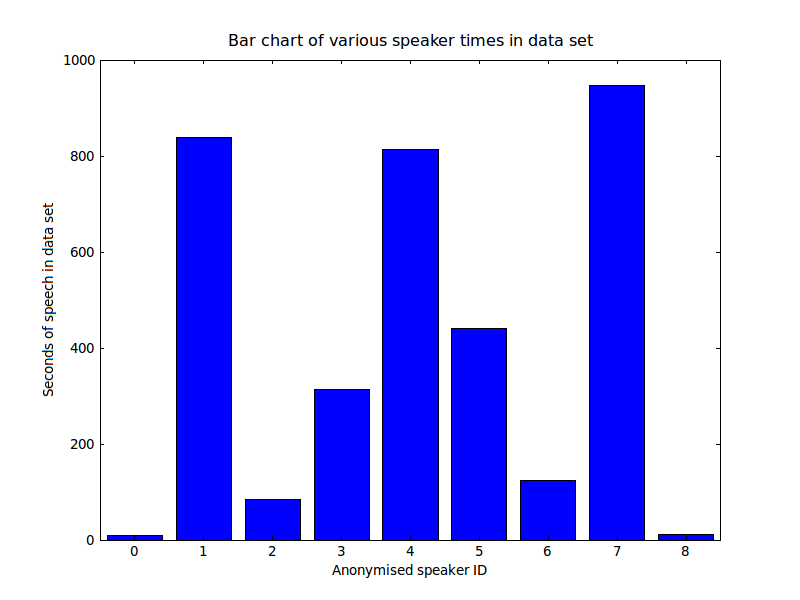
\includegraphics[height=10cm]{speaker.png}
    \label{img:speaker_distribution}
    \caption{Distribution of speakers in the labelled dataset}
\end{figure}

\begin{figure}
    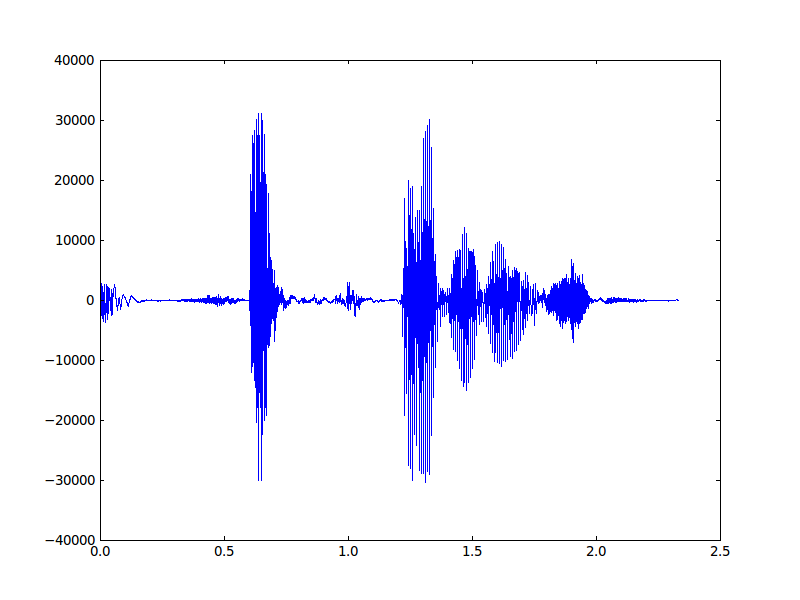
\includegraphics[width=8cm]{labelling1.png}
    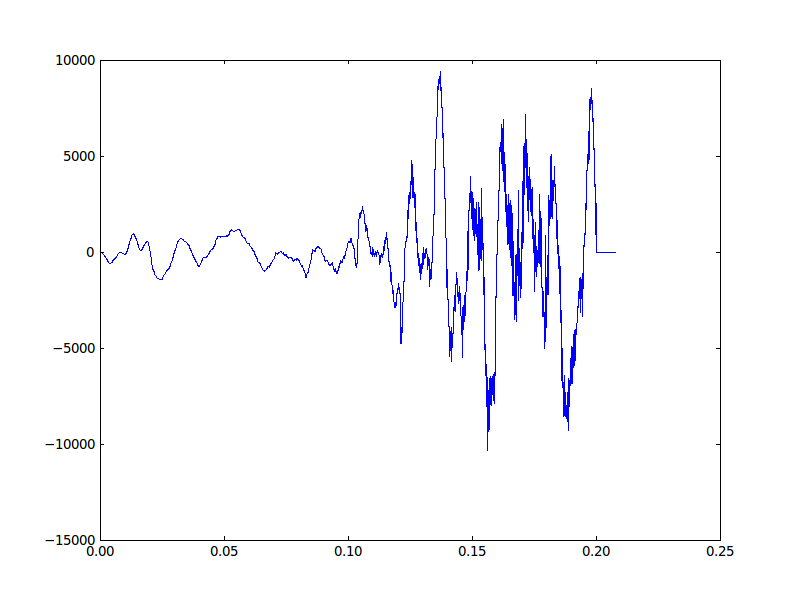
\includegraphics[width=8cm]{labelling2.png}
    \label{img:labelling_example}
    \caption{Example of contiguous and short region in simple labelling system}
\end{figure}

\section{Building the classifier}

From the start we used the Random Forest classifier discussed in section
\ref{section:random-forest}, this is due to both familiarity, and availability.
Specifically we took an off the shelf implementation from the
scikit-learn\cite{sklearn} Python library. This library was chosen due to it's
general popularity and the author's familiarity with python. Once the
classifier had been chosen we decided to act on windows of 16ms, this number
was chosen because it is used in gaming applications as the target framerate of
any on screen graphics, corresponding to 60 frames per second, which most
players perceive to be acting in real time. The background research indicates
that this frame size is not outside the desired range of 10-30ms, it is worth
however noting that the Shin\cite{shin} system uses a slightly shorter, 10ms
window size.

In this section, classification accuracies are reported as the result of a 10
fold, randomised, stratified cross validation (there was a minor imbalance in
the number of samples in each of the classes, with roughly 53\% background
noise and 47\% voice). The folds were trained with 66\% of the data in the
training set, we felt that this split gives a reasonable tradeoff between
giving the classifier sufficient data to train on, and not training in such a
way that the classifier would be overly biased towards the dataset, in other
words we are trying to retain some of the generalizability of our classifier by
using a 66\% training set rather than a 90\% training set.

The general binary classification problem that we formulated in the technical
background chapter of this paper requires that we have some fixed size vector
of real numbers for each sample in the training/test sets, obviously this means
that we cannot pass some arbitrary length audio stream into the classifier and
attempt to build a result, so the natural thing to do is to apply a "windowing"
to the audio. Specifically: we must pick a fixed window size that is short
enough that it will not be perceived as lagging whilst classification is
occurring, short enough that we can classify it in real time (if our window
contains 1 million samples it is unlikely that we can classify it in real
time), and long enough that it contains enough information so that it can be
classified.

We initially chose a 16ms window size as the size of the window for
classification, this falls within the common window sizes in the background
literature, which typically fall in the 10ms-30ms, and our specific choice of
16ms was made because this is the traditional framerate that many gaming
applications target, representing 60 frames a second, traditionally perceived
as smooth by most gamers. In chapter \ref{chap:evaluation} we assess the
relative merits of window sizes in the 10-30ms range, and the affects those
have on classification accuracy. Our initial choice of 16ms, with the 48000Hz
audio that we use gives us 768 samples per window. Initially we decided to pass
all 768 samples as a vector as the representation of the window for
classification.

The classifier with 768 samples gave a relatively unsatisfying classification
accuracy of around 77\%. It was obvious that the raw samples were not amenable
to classification due to the position of individual windows having very little
with the actual audio that was happening, and more importantly each frame
within the 16ms window basically took every value regardless of class, so we
began to implement features from the background research to begin to improve
classification accuracy.

In order to allow easy construction of a representation of the audio that would
allow for a high classification accuracy, we added another stage to the
pipeline that sat between the audio on the hard drive and the classifier.
Specifically the pipeline had these stages:

\begin{itemize}

    \item For reach row of the database, extract class label, start time, end time
        and file name

    \item For each of those, open the file for reading and read samples out of
        the file between the start time and the end time

    \item Cut the sample into 16ms windows, appending 0s if necessary.

    \item Apply all feature transforms to get a uniform width vector of integers

    \item Send feature vectors along with class labels into the classifier for
        training.

\end{itemize}

This allowed us to mix feature transformations as the project went on, removing
and adding as necessary. The features that were initially implemented were
based on the research and also some visualization/analysis of the dataset. The
initial feature set we went with was:

\begin{enumerate}
    \item Energy: the sum of squares of the frame, referred to in the technical
        background chapter.

    \item Zero crossing rate: the number of times the samples in the frame
        change in sign, referred to in the technical background chapter.

    \item The energy of the 3500 to 4300Hz frequency band: implemented as a
        squared sum of the fourier magnitude domain of the values in this
        frequency band. This feature was implemented due to it corresponding to
        a peak in the average fourier transform of one of the classes

    \item The energy of the 5400 to 6800Hz frequency band: implemented as above,
        This feature was implemented due to it corresponding to a peak in the
        average fourier transform of one of the classes.

    \item The energy of the 1800 to 2700Hz frequency band: this corresponds to
        the most dominant frequencies of voice according to the research

    \item The dominant frequency in the 300 to 5000Hz band: this is a wide band
        around the fundamental frequency of human voice, up to a very high harmonic,
        in an attempt to differentiate keyboard noise from voice.

    \item The energy in the 0-100Hz energy band: this band was chosen
        due to the effects of windowing on the fourier-amplitude domain and is discussed
        further in this section.

    \item The kurtosis of the fourier-amplitude domain: this is effectively a
        measure of "peakyness" of the spectrum and will be discussed further
        in this section.


    \item The residual from a p=12 lpc analysis: as discussed in the technical
        background chapter, the lpc has been shown to be a good predictor of
        voice signals, with p much lower than the period of the voice signal.
        The residual is computed as the squared error of the LPC over the window.

    \item The 12 coefficients of a p=12 pole lpc analysis: these coefficients
        give a different view on the result of the LPC from the residual. Our
        fear with this feature was that they may have a high level of
        covariance. But in \ref{fig:covariance-lpc} we can see that there is
        blah

    \item The third component of the power spectral density of the signal: this
        component corresponds to a large speak in the average power spectrum,
        which can be seen in \ref{fig:psd}.

    \item The dominant component of the power spectal density of the signal
        above the third component: this feature was determined experimentally
        to be a reasonable weak estimator that separates our negative and
        positive classes.

    \item The sum of the power spectral densities between the 30th and 37th components:
        this feature was determined experimentally to help classification as much
        as any of the other features.

    \item The energy at another peak (21st component) within the PSD of the signal:
        this was also determined experimentally to provide reasonable classification
        accuracy on our problem set.

\end{enumerate}

Features 2, 3, 4 and 7 are shown along with the complete fourier amplitude domain
in \ref{fig:frequencies}

\begin{figure}
    \label{fig:frequencies}
    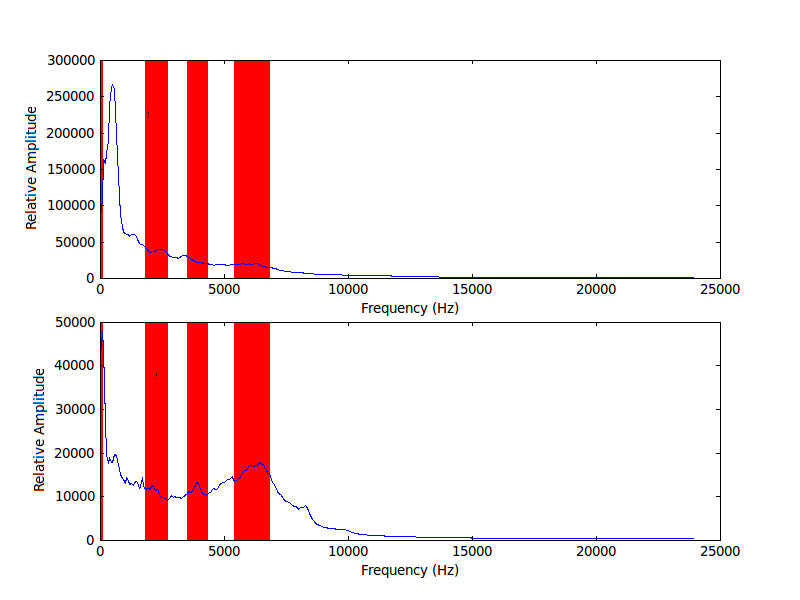
\includegraphics[height=10cm]{frequencies.png}
    \caption{Histogram of fourier domain for voice and noise classes, voice
    at the top, and noise at the bottom, with the frequency bands highlighted}
\end{figure}

As we can see these three frequency bands vary from each other between the two
classes, specifically we can see that these frequency bands represent spikes in
the noise class, that are more flat in the voice class, and in addition that
the relative amplitude at these points is much, much lower for the noise class
than the voice, class. In \ref{table:importances} we show the relative feature
importances as computed by the classifier over our original feature set. These
give relatively high importances (specifically just over 11\% of
the classification accuracy come from the 3 higher frequency bands).

\begin{figure}
    \label{table:importances}
    \begin{tabular}{| l | l |}
    \hline
        Feature                                    & Normalized Importance \\ \hline
        1800-2700Hz band energy                    & 0.054 \\
        3500-4300 band energy                      & 0.036 \\
        5400-6800 band energy                      & 0.022 \\
        dominant frequency (300-5000Hz)            & 0.028 \\
        window energy                              & 0.057 \\
        kurtosis of the fft                        & 0.028 \\
        0-100Hz band energy                        & 0.187 \\
        lpc coefficient \#0                        & 0.046 \\
        lpc coefficient \#1                        & 0.029 \\
        lpc coefficient \#10                       & 0.019 \\
        lpc coefficient \#11                       & 0.018 \\
        lpc coefficient \#2                        & 0.043 \\
        lpc coefficient \#3                        & 0.028 \\
        lpc coefficient \#4                        & 0.024 \\
        lpc coefficient \#5                        & 0.019 \\
        lpc coefficient \#6                        & 0.018 \\
        lpc coefficient \#7                        & 0.016 \\
        lpc coefficient \#8                        & 0.018 \\
        lpc coefficient \#9                        & 0.019 \\
        lpc residual                               & 0.041 \\
        PSD peak at 21st component                 & 0.032 \\
        PSD dominant component after 3rd component & 0.017 \\
        the third PSD component                    & 0.109 \\
        the sum of 30th-37th PSD components        & 0.038 \\
        zero crossings                             & 0.044  \\
    \hline
    \end{tabular}
\end{figure}

The importances are computed by the random forest classifier during training
and reported once tranining is complete. They are computed as a function of
depth of the feature within each tree, and the relative fraction of instances
that can be accurately split by that feature. These importances are then
averaged accross the entire forest. From this we can get a relative ranking and
importance value from the features. We can see here that two of our features
(0-100Hz dominant frequency and third PSD component) account for approximately
30\% of the importance of the classifier, while the rest of the features all
have roughly the same importance, ranging from 1.6\% to 5.4\% relative
importanca.

One of the most interesting things that this indicates is that the
energy of the audio windows is not a good feature to classify with on our
particular dataset. This result is somewhat unexpected as classification energy
has typically been the single most used feature that we could find in our
research. The cause for the relatively low importance of the energy feature in
our data set will be due to the slightly different nature of the problem:
energy deals specifically with the perceived loudness of a frame, and in our
data set, the frames with keyboard noise have roughly equal amplitude to the
frames that have human speech in them.

The zero crossing rate similarly performs as one of the lower accuracy
features. This feature was also found commonly in the background research, and
more specifically has been shown to be a good feature for classifying
percussion \cite{gouyon}. Given that keyboard noise is generated in a similar
way to percussion in music (a fast impact on to a surface) we expected this
feature to provide a much better importance, this can perhaps be explained by
noting that the zero crossing rates between keyboards and voice may be similar
whilst the crossing rates between keyboards and voice, and background noise may
be very different.

The explanation for the very high level of classification importance provided
by the 0-100Hz band energy comes from the windowing process: the lower
frequency information of the fourier transform is naturally amplified by the
windowing process and this is the explanation for why the fourier transform
shows such a high spike for both classes in this region. We can see more
clearly, however, that in \ref{fig:frequencies} the average fourier transform
has a dip for the voice class in this frequency band, but a spike for the noise
class in this frequency band, this, we believe, accounts for the reason why
this feature splits the highest fraction of samples in our data set.

The reason for the third PSD component also giving this very accurate
classification is that it speaks for roughly the same part of the spectrum as
the energy band in 0-100Hz. Based off this finding we also tried a composite
feature: the sum of the PSD components 0-3 as opposed to just the 3rd
component. This gave a slightly improved classification accuracy: 91\% in
cross val versus 90\% and so our updated feature set used the sum of the band
instead of the single value.

Whilst the majority of the heavy lifting of the classification is done by these
two features (accounting for correctly classifying 30\% of the samples). The
remaining 70\% comes from the composite interaction of the remainder of our
features. To get an understanding as to whether any of these features interact
with each other, we decided it would be useful to build a matrix of feature
correlations. If any features are highly correlated then it would suggest that
these features do not give us as much useful information as if they were highly
anti-correlated.

\begin{sidewaystable}
    \begin{tabular}{|c|c|c|c|c|c|c|c|c|c|c|c|c|}
        \hline
           & 1      & 2      & 3      & 4      & 5      & 6      & 7      & 8      & 9      & 10     & 11     & 12     \\ \hline
        1  & 1.000  & 0.429  & 0.136  & -0.013 & 0.370  & -0.067 & 0.013  & -0.027 & 0.093  & -0.025 & -0.010 & -0.027 \\ \hline
        2  & 0.429  & 1.000  & 0.321  & 0.124  & 0.304  & -0.083 & 0.023  & 0.090  & 0.099  & -0.033 & -0.003 & -0.081 \\ \hline
        3  & 0.136  & 0.321  & 1.000  & 0.220  & 0.209  & -0.103 & 0.003  & 0.248  & 0.096  & -0.030 & 0.013  & -0.079 \\ \hline
        4  & -0.013 & 0.124  & 0.220  & 1.000  & -0.092 & -0.324 & -0.038 & 0.636  & 0.411  & -0.162 & -0.098 & -0.378 \\ \hline
        5  & 0.370  & 0.304  & 0.209  & -0.092 & 1.000  & 0.064  & 0.399  & -0.116 & 0.067  & 0.045  & 0.061  & 0.166  \\ \hline
        6  & -0.067 & -0.083 & -0.103 & -0.324 & 0.064  & 1.000  & 0.094  & -0.468 & -0.445 & 0.033  & 0.013  & 0.409  \\ \hline
        7  & 0.013  & 0.023  & 0.003  & -0.038 & 0.399  & 0.094  & 1.000  & -0.048 & -0.077 & -0.006 & 0.007  & 0.046  \\ \hline
        8  & -0.027 & 0.090  & 0.248  & 0.636  & -0.116 & -0.468 & -0.048 & 1.000  & 0.350  & -0.100 & 0.014  & -0.556 \\ \hline
        9  & 0.093  & 0.099  & 0.096  & 0.411  & 0.067  & -0.445 & -0.077 & 0.350  & 1.000  & -0.070 & -0.031 & -0.397 \\ \hline
        10 & -0.025 & -0.033 & -0.030 & -0.162 & 0.045  & 0.033  & -0.006 & -0.100 & -0.070 & 1.000  & 0.614  & -0.040 \\ \hline
        11 & -0.010 & -0.003 & 0.013  & -0.098 & 0.061  & 0.013  & 0.007  & 0.014  & -0.031 & 0.614  & 1.000  & -0.036 \\ \hline
        12 & -0.027 & -0.081 & -0.079 & -0.378 & 0.166  & 0.409  & 0.046  & -0.556 & -0.397 & -0.040 & -0.036 & 1.000  \\ \hline
        13 & 0.004  & 0.052  & 0.144  & 0.299  & -0.015 & -0.211 & -0.017 & 0.401  & 0.059  & -0.149 & -0.080 & -0.170 \\ \hline
        14 & -0.048 & -0.022 & -0.016 & 0.094  & 0.014  & -0.051 & -0.003 & -0.044 & 0.078  & 0.063  & -0.110 & -0.077 \\ \hline
        15 & -0.007 & 0.028  & 0.068  & 0.005  & 0.024  & 0.015  & -0.005 & -0.086 & -0.066 & 0.061  & -0.012 & 0.066  \\ \hline
        16 & 0.005  & 0.009  & 0.007  & -0.177 & 0.074  & 0.121  & 0.009  & -0.250 & -0.153 & 0.077  & 0.078  & 0.203  \\ \hline
        17 & 0.072  & 0.034  & 0.001  & -0.101 & -0.140 & -0.051 & 0.072  & 0.084  & 0.175  & -0.159 & -0.006 & 0.518  \\ \hline
        18 & 0.018  & 0.004  & -0.003 & -0.180 & 0.076  & 0.028  & -0.007 & -0.109 & -0.145 & 0.242  & 0.013  & 0.025  \\ \hline
        19 & 0.029  & 0.020  & 0.029  & -0.132 & 0.085  & -0.019 & -0.004 & -0.031 & -0.082 & 0.608  & 0.254  & -0.055 \\ \hline
        20 & 0.072  & 0.123  & 0.090  & -0.001 & 0.161  & -0.003 & 0.261  & 0.025  & -0.023 & -0.009 & 0.001  & 0.005  \\ \hline
        21 & 0.168  & 0.685  & 0.141  & 0.076  & 0.142  & -0.034 & 0.009  & 0.046  & 0.054  & -0.028 & -0.013 & -0.044 \\ \hline
        22 & -0.027 & 0.077  & 0.195  & 0.571  & -0.113 & -0.296 & -0.018 & 0.780  & 0.363  & -0.100 & -0.010 & -0.519 \\ \hline
        23 & 0.151  & 0.090  & -0.003 & -0.118 & 0.735  & 0.103  & 0.683  & -0.135 & -0.028 & 0.036  & 0.042  & 0.138  \\ \hline
        24 & 0.122  & 0.289  & 0.946  & 0.205  & 0.197  & -0.094 & 0.002  & 0.234  & 0.089  & -0.029 & 0.012  & -0.072 \\ \hline
        25 & -0.026 & 0.078  & 0.202  & 0.590  & -0.182 & -0.550 & -0.077 & 0.890  & 0.246  & -0.065 & -0.010 & -0.609 \\ \hline
    \end{tabular}
\end{sidewaystable}
\begin{sidewaystable}

    \begin{tabular}{|c|c|c|c|c|c|c|c|c|c|c|c|c|c|c|c|}
        \hline
           & 13     & 14     & 15     & 16     & 17     & 18     & 19     & 20     & 21     & 22     & 23     & 24     & 25 \\ \hline
        1  & 0.004  & -0.048 & -0.007 & 0.005  & 0.020  & 0.018  & 0.029  & 0.072  & 0.168  & -0.027 & 0.151  & 0.122  & -0.026 \\ \hline
        2  & 0.052  & -0.022 & 0.028  & 0.009  & 0.023  & 0.004  & 0.020  & 0.123  & 0.685  & 0.077  & 0.090  & 0.289  & 0.078 \\ \hline
        3  & 0.144  & -0.016 & 0.068  & 0.007  & 0.039  & -0.003 & 0.029  & 0.090  & 0.141  & 0.195  & -0.003 & 0.946  & 0.202 \\ \hline
        4  & 0.299  & 0.094  & 0.005  & -0.177 & -0.174 & -0.180 & -0.132 & -0.001 & 0.076  & 0.571  & -0.118 & 0.205  & 0.590 \\ \hline
        5  & -0.015 & 0.014  & 0.024  & 0.074  & 0.072  & 0.076  & 0.085  & 0.161  & 0.142  & -0.113 & 0.735  & 0.197  & -0.182 \\ \hline
        6  & -0.211 & -0.051 & 0.015  & 0.121  & 0.034  & 0.028  & -0.019 & -0.003 & -0.034 & -0.296 & 0.103  & -0.094 & -0.550 \\ \hline
        7  & -0.017 & -0.003 & -0.005 & 0.009  & 0.001  & -0.007 & -0.004 & 0.261  & 0.009  & -0.018 & 0.683  & 0.002  & -0.077 \\ \hline
        8  & 0.401  & -0.044 & -0.086 & -0.250 & -0.101 & -0.109 & -0.031 & 0.025  & 0.046  & 0.780  & -0.135 & 0.234  & 0.890 \\ \hline
        9  & 0.059  & 0.078  & -0.066 & -0.153 & -0.140 & -0.145 & -0.082 & -0.023 & 0.054  & 0.363  & -0.028 & 0.089  & 0.246 \\ \hline
        10 & -0.149 & 0.063  & 0.061  & 0.077  & -0.051 & 0.242  & 0.608  & -0.009 & -0.028 & -0.100 & 0.036  & -0.029 & -0.065 \\ \hline
        11 & -0.080 & -0.110 & -0.012 & 0.078  & 0.072  & 0.013  & 0.254  & 0.001  & -0.013 & -0.010 & 0.042  & 0.012  & -0.010 \\ \hline
        12 & -0.170 & -0.077 & 0.066  & 0.203  & 0.084  & 0.025  & -0.055 & 0.005  & -0.044 & -0.519 & 0.138  & -0.072 & -0.609 \\ \hline
        13 & 1.000  & 0.089  & -0.124 & -0.058 & 0.175  & 0.104  & 0.015  & -0.002 & 0.016  & 0.188  & -0.042 & 0.135  & 0.316 \\ \hline
        14 & 0.089  & 1.000  & 0.243  & -0.069 & -0.159 & 0.122  & 0.125  & -0.006 & -0.013 & -0.096 & 0.009  & -0.013 & -0.045 \\ \hline
        15 & -0.124 & 0.243  & 1.000  & 0.406  & -0.006 & -0.125 & 0.056  & -0.008 & 0.010  & -0.149 & -0.005 & 0.065  & -0.076 \\ \hline
        16 & -0.058 & -0.069 & 0.406  & 1.000  & 0.518  & 0.144  & -0.069 & -0.002 & -0.003 & -0.267 & 0.035  & 0.008  & -0.234 \\ \hline
        17 & 1.000  & 0.554  & 0.163  & -0.007 & -0.005 & -0.176 & 0.023  & 0.038  & -0.105 & 0.123  & 0.012  & -0.113 & 0.015\\ \hline
        18 & 0.104  & 0.122  & -0.125 & 0.144  & 0.554  & 1.000  & 0.591  & -0.006 & -0.015 & -0.166 & 0.034  & -0.001 & -0.078 \\ \hline
        19 & 0.015  & 0.125  & 0.056  & -0.069 & 0.163  & 0.591  & 1.000  & 0.003  & -0.008 & -0.093 & 0.044  & 0.027  & -0.029 \\ \hline
        20 & -0.002 & -0.006 & -0.008 & -0.002 & -0.007 & -0.006 & 0.003  & 1.000  & 0.048  & 0.042  & 0.106  & 0.087  & 0.004 \\ \hline
        21 & 0.016  & -0.013 & 0.010  & -0.003 & -0.005 & -0.015 & -0.008 & 0.048  & 1.000  & 0.045  & 0.042  & 0.133  & 0.044 \\ \hline
        22 & 0.188  & -0.096 & -0.149 & -0.267 & -0.176 & -0.166 & -0.093 & 0.042  & 0.045  & 1.000  & -0.099 & 0.186  & 0.680 \\ \hline
        23 & -0.042 & 0.009  & -0.005 & 0.035  & 0.023  & 0.034  & 0.044  & 0.106  & 0.042  & -0.099 & 1.000  & -0.004 & -0.185 \\ \hline
        24 & 0.135  & -0.013 & 0.065  & 0.008  & 0.038  & -0.001 & 0.027  & 0.087  & 0.133  & 0.186  & -0.004 & 1.000  & 0.190 \\ \hline
        25 & 0.316  & -0.045 & -0.076 & -0.234 & -0.105 & -0.078 & -0.029 & 0.004  & 0.044  & 0.680  & -0.185 & 0.190  & 1.000 \\ \hline
    \end{tabular}
\end{sidewaystable}

\begin{figure}
    \begin{tabular}{ |l|l| }
        Table Heading & Label Number \\
        1800 to 2700Hz Band energy & 1 \\
        3500 to 4300Hz Band energy & 2 \\
        5400 to 6800HZ Band Energy & 3 \\
        Dominant Frequency in the 300 to 5000 Hz band & 4 \\
        Energy of the window & 5 \\
        Kurtosis of the fft & 6 \\
        0 to 100Hz Band Energy & 7 \\
        LPC Component 0 & 8 \\
        LPC Component 1 & 9 \\
        LPC Component 10 & 10 \\
        LPC Component 11 & 11 \\
        LPC Component 2 & 12 \\
        LPC Component 3 & 13 \\
        LPC Component 4 & 14 \\
        LPC Component 5 & 15 \\
        LPC Component 6 & 16 \\
        LPC Component 7 & 17 \\
        LPC Component 8 & 18 \\
        LPC Component 9 & 19 \\
        LPC Residual & 20 \\
        Peak at 21st PSD component & 21 \\
        PSD dominant component after third component & 22 \\
        Sum of PSD components 0 through 3 & 23 \\
        Sum of PSD components 30 through 36 & 24 \\
        Zero Crossing rate 25 & \\
    \end{tabular}
    \caption{Table of features to integer key mappings}
    \label{fig:feature-keys}
\end{figure}

From these tables we can see that there is a very low level of correlation
between most of the features: the average correlation is (blah) and the
standard deviation is (blah).

However, some of these variables are highly correlated. This suggests that
perhaps we could remove these features or perform a principal component
analysis to further reduce the dimensionality of the data. Specifically:

\begin{itemize}

    \item 16 and 17 have a correlation of just over 0.5. These features
        represent the 6th and 7th components of the LPC analysis. This result
        is not entirely unexpected as the LPC attempts to best fit the signal,
        in some signals (such as flat noise) there is very little variation
        needed to predict the next item from the previous 12.

    \item 6 and 25 have a correlation of -0.550. This is a relatively strong
        negative correlation. The kurtosis of the FFT and the zero crossing
        rate are somewhat inherently linked as the whole spectrum of the signal
        will determine the zero crossing rate, and the kurtosis is a summary
        statistic of the FFT.

    \item 8 and 22 have a correlation of 0.780. The 0th LPC coefficient and the
        dominant component of the PSD after the third component are possibly
        linked in that the LPC coefficient will change with frequency
        information and the dominant frequency is obviously directly extracting
        frequency information

    \item 8 and 25 have a correlation of 0.890. The 0th LPC coefficient and the
        zero crossing rate are inherently linked: the zero crossing rate describes
        a characteristic that the LPC is trying to accurately predict, that is the
        rate of sign change in the signal.
\end{itemize}

Checking these feature correlations during building the system was useful, if a
new feature provided a low gain in either classifier importance or had high correlations
with other features we could easily reject them. This way we were able to reject
a number of features from our implementation. We have documented these below with
reasons for their rejection.

\begin{itemize}

    \item The mean value of frames in the window. This was found to have very
        poor predictive importance, even with fewer features.  This is
        especially bad as predictive importance is normalized to sum to 1
        regardless of the feature count.  Specifically the predictive
        importance was: 0.1\%, some 10$times$ smaller than even our worst
        predictive importances.

    \item The spectral flatness measure of the power spectrum: in the technical
        background neasure we indicated that the LPC residual is equivalent to
        the spectral flatness measure of the absolute values of the fourier
        transform. Whilst the power spectrum does differ from the frequency
        spectrum it is somewhat correlated, and as such the SFM of the power
        spectrum was highly correlated (r=0.841) with the LPC residual energy.

    \item The energy of the 2-4Khz band. Whilst this feature was used in
        \cite{shin} we found that this feature did not give good predictive
        power.  This feature was actually implemented before the energy bands
        that we used but we found that the bands that we decided on gave better
        predictive power for our problem set. We believe this is due to both voice
        harmonics and keyboard noise occupying this frequency band.

    \item The dominant frequency of the entire spectrum. This feature was
        originally implemented in an attempt to increase classification
        accuracy, however based on the spectra in \ref{fig:frequencies} the
        problem with this feature becomes obvious: due to the windowing process
        much of the low frequency information gets overly represented. This
        means that this feature would always stop above the 200Hz value. The
        features we ended up using specifically take into account this spike
        and attempt to give a much better representation of the dominant
        frequencies in the signal.

    \item After the features that have been described above were implemented in
        the system we investigated adding cepstral features into the system, we
        did, however, find that the features from the cepstrum were already
        accounted for in the rest of our features, and that they were
        correlating highly with many of the other features in the classifier
        without providing particularly high feature importances from the classifier, and
        as such they were rejected.

    \end{itemize}

\section{Analysis of the features with respect to accuracy}

Once we had built the random forest classifier and tested the features that we
had, investigated further features and rejected some along the way, the next
step in our implementation was to determine the absolute predictive power of
our features. In order to do this we trained decision trees on each feature
individually: the objective of this exercise was to determine how accurately
the feature importances reported from the classifier represent the predictive
power of the individual features, and also to show how much stronger the
predictive power of the combination of all the features is than any individual
feature. Another objective here is to demonstrate that the combination of
features that we have designed perform significantly better than merely
training a classifier on the entire audio frame.

The reports of accuracy here are given by taking the results of a 10 fold, 66\%
training, 33\% test cross validation. Accuracy was determined using the MAE
metric and the standard deviation in this metric also reported. The features
here are keyed the same as the mappings in \ref{fig:feature-keys}.

\begin{figure}
    \begin{tabular}{|l|l|l|}
        1 & 0.61125383971 & 0.00185529016944 \\ \hline
        2 & 0.576193800614 & 0.00441615026379 \\ \hline
        3 & 0.542711533091 & 0.00285376833334 \\ \hline
        4 & 0.603965372801 & 0.00307252916356 \\ \hline
        5 & 0.625174532254 & 0.00175006337411 \\ \hline
        6 & 0.530522200503 & 0.00631432897544 \\ \hline
        7 & 0.706311086289 & 0.00240115788572 \\ \hline
        8 & 0.578790840547 & 0.00304710722648 \\ \hline
        9 & 0.539276738341 & 0.00432177385115 \\ \hline
        10 & 0.51227310807 & 0.00196242563343 \\ \hline
        11 & 0.507735269478 & 0.00440018483912 \\ \hline
        12 & 0.554984641162 & 0.00286100050223 \\ \hline
        13 & 0.518584194359 & 0.00395399960351 \\ \hline
        14 & 0.520650656241 & 0.00268662685748 \\ \hline
        15 & 0.518304942753 & 0.00303710996038 \\ \hline
        16 & 0.514981848646 & 0.00133749567326 \\ \hline
        17 & 0.512552359676 & 0.00486759660219 \\ \hline
        18 & 0.514632784139 & 0.00491288422114 \\ \hline
        19 & 0.507442055292 & 0.0020289507721 \\ \hline
        20 & 0.609522479754 & 0.00315609912735 \\ \hline
        21 & 0.561239877129 & 0.00412626730991 \\ \hline
        22 & 0.601689472214 & 0.00209652687857 \\ \hline
        23 & 0.675439821279 & 0.00122441559723 \\ \hline
        24 & 0.548994694219 & 0.00162074225464 \\ \hline
        25 & 0.705696732756 & 0.00150485267638 \\ \hline
    \end{tabular}
    \caption{Table showing the relative accuracies of individual features}
\end{figure}

As we can see the 0-100Hz band energy feature is by far the best predictor
within the indivudal feature set. This corresponds strongly with the feature
importances computed by the classifier. An interesting upset is that feature 25
also gives a relatively high prediction rate on it's own, but the zero crossing
rate was one of the features given the lowest importance by the classifier that
uses all the features. This is particularly interesting because according to
the correlation matrix of features, 7 and 25 are relatively uncorrelated
(-0.077), as such if they both have strong predictive power, we would expect them
to combine together to give a much better classification accuracy.

It is worth noting that our second best predictor from the importances in
\ref{table:importances}, the sum of the first 4 (0-3 inclusive) PSD components
comes a very close third in this table, with 68.5\% accuracy as a predictor on
it's own. The reason that our classification rate is so much higher than any
individual feature combined is that, whilst each of the individual features may
not have much better prediction accuracy than the baseline, they are all
somewhat uncorrelated, meaning that they present different views on the data
and as such allow the random forest classifier to extract nearly all of the
variance from the data set and provide a much more accurate classification.

%-----------------------------------
%-----------------------------------
%-----------------------------------
%-----------------------------------
%-----------------------------------
%-----------------------------------
%-----------------------------------
%-----------------------------------

\chapter{Critical Evaluation}
\label{chap:evaluation}

{\bf A topic-specific chapter, of roughly $10$ pages}
\vspace{1cm}

In this chapter we have given the results of a number of experiments that were
performed over our classifier built in the previous chapter, with regards to
various facets such as classification accuracy, performance and
generalizability.

\section{Sample Bits}

In the technical background chapter we explained how each sample of audio is
represented by a number of bits, more bits giving much higher fidelity audio
recreation. We started with 16 bit audio samples, and in this experiment we
investigate the affect of changing to 8 bits per sample instead. There are a
number of compelling reasons to make this change:

\begin{enumerate}

    \item If the bits per sample can be reduced, the overall data rate going
        through the system will be reduced, this may give performance benefits
        such as being able to apply the feature transformations more quickly,
        and fitting more data in the cache lines. Particularly as VAD systems
        are used in embedded/mobile computing contexts, being able to work with
        smaller data sets is important.

    \item Additionally it means that the data set that we use can be more
        aggressively compressed for serving on the internet: we have built a
        unique corpus that includes audio like laughter and keyboard noise
        which were not found in the existing literature, and as such distributing
        the data set more easily is a benefit.

\end{enumerate}

We obviously expect to see a reduced classification accuracy from cutting out
the lower 8 bits of audio information, but it is worth noting that unlike
music, voice tends to have a fairly uniform amplitude, and so the minor
variations may not have that much of an effect.

To perform this experiment, we modified the part of the program that reads the
audio from the files, and instead of just passing out the entire audio sample
we masked out the lower 8 bits of the 16 bit sample, to get an initial
indication of how much of an affect removing these bits would have on the
accuracy of the classification system. In order to perform testing, we trained
our classifier system on 50\% of the data in the training set, testing against
the over 50\% and plotted the roc curves which are shown in \ref{fig:roc-bitcrush}

\begin{figure}
    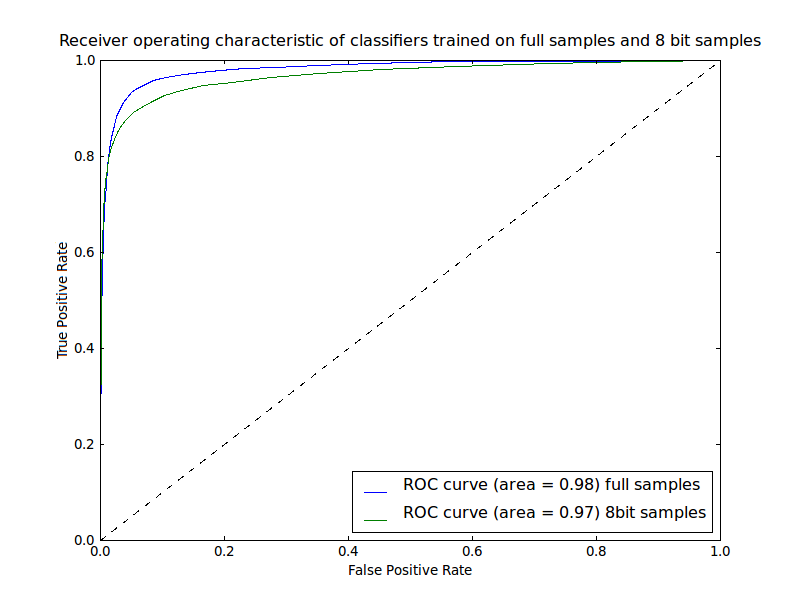
\includegraphics[height=10cm]{roc_8bit.png}
    \caption{ROC curves of the two classifiers}
    \label{fig:roc-bitcrush}
\end{figure}

This curve clearly shows that the accuracy of the two classifiers is nearly the
same (98\% area under the ROC curve for the full bit samples, versus 97\% area
under the ROC curve for 8 bit samples). This finding is useful, it means that
the classifier can be trained on smaller data sets, reducing the overall size
of the classification model that has to be loaded into memory: the full
classifier takes 65 megabytes of memory, the reduced one takes only 40. This
means that, for example, this system could be released on both PC and embedded
contexts, with the slightly higher accuracy version being released on PC and
the lower accuracy version released on the embedded/mobile devices. One of the
main aims of this project is to release our corpus after we have completed, and
it is important to note that reducing the size of the archive that we release
will directly increase the number of people that it is available to. By halfing
the bitrate (by reducing the number of bits per frame) we think this result is
genuinely a good way to improve our ability to release the system, and improve
performance.

\section{Frame Rate}

Changing the frame rate will naturally be expected to alter classifier accuracy
and performance: firstly having to work with fewer frames will mean that the
fourier transforms that we use are more sparse, and that we have to work over
less data when computing features like the energy of the frame. This may also
lead to a reduced classification accuracy. There is some reason to believe that
this may not have as much impact as changing the bit rate of the classifier,
this is due to the fact that human voice rarely goes above 4000Hz, with a
nyquist limit of 8000Hz. Our audio samples being recorded at 48000Hz means
that we may have vastly much more information than we need. In order to test
this we initially started by taking half (24000Hz) and quarter (12000Hz) frame
rates, to determine whether or not this would have a significant affect on
classification accuracy. The results are shown in \ref{fig:roc-frameratecrush}.

\begin{figure}
    \label{fig:roc-frameratecrush}
    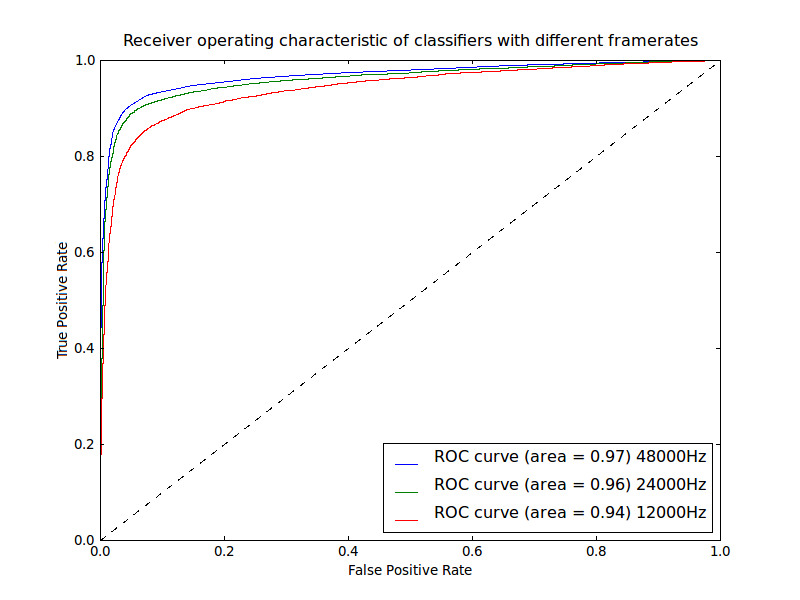
\includegraphics[width=15cm]{roc_framerates.png}
    \caption{ROC curves for various reduced framerates}
\end{figure}

\section {Robustness to unseen data}

\subsection{Unseen speakers}
There are multiple ways we can pass unseen data to our classifier, having been
trained on only 9 speakers there is a possibility that it will not work well
with new people. To test this we recorded a sequence of audio containing pure
speech/silence (no strong keyboard impulses) from an unseen, male, speaker of
approximately 16.5 seconds in length. This gave us 1037 windows to classify
against the unseen speaker. Whilst this is a short amount of audio, the
labelling process for this being the limiting factor in our ability to create a
large window of audio to classify against. The classifier was trained against
the entire labelled training set that we created, and then classification was
performed on each of the frames in the sequence provided. The confusion matrix
for this experiment can be seen in \ref{table:confusion_unseen}, it should be
noted that any 16ms window with total silence is discarded, so only 822
actually got classified. From a visual inspection of the data in
\ref{fig:waveform_unseen} we can see that noise regions were correctly classified, with
only a few frames getting through, but most voice regions were classified
noisily. In order to improve this system to generalize better to unseen
speakers, we would require a much much larger sample of audio to draw from, but
again hand labelling may significantly slow the process.


\begin{figure}
    \label{table:confusion_unseen}
    \begin{center}
        \begin{tabular}{| l | l | l |}
            \hline
            & Predicted Voice & Predicted Noise \\ \hline
            Actual Voice & 43 & 123 \\
            Actual Noise & 40 & 616 \\ \hline
        \end{tabular}
    \end{center}
    \vspace{\baselineskip}

    The confusion matrix indicates that the classification is very good at
    classifying background noise, but not so good at classifying speech. This
    result is expected: it indicates that there is much more variation in the
    voice of an unseen speaker than the background noise of an unseen
    configuration. This is due to the fact that addative background noise is
    largely the same in any environment, and it being picked up is largely due
    to the different sensitivities of microphones.

    \caption{Confusion matrix for unknown speaker}
\end{figure}

\begin{figure} 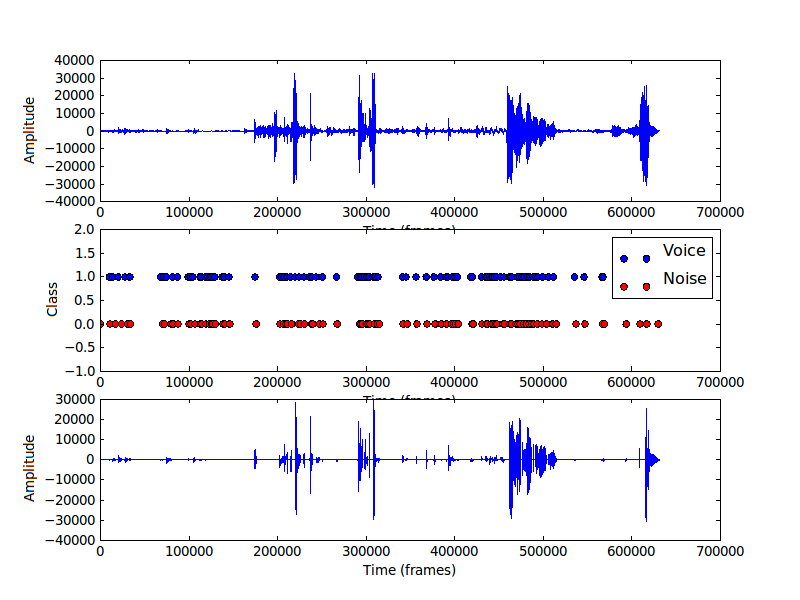
\includegraphics[width=10cm]{peter.png}
    \label{fig:waveform_unseen}

    This diagram shows the waveform, class over
    time, and post-processed waveform for a specific audio sequence. The middle
    diagram, which shows class represents the classification of each specific
    window over time, only showing class when a change occurs. We can see here
    that the classification on an unseen speaker with unseen data is very very
    noisy when in the speech class, and somewhat accurate in the noise class.
    This suggests that the background noise detection in the classifier is
    reasonably accurate, and the detector for voice is not so robust to unseen
    voice data. A possible explanation for this is that there is significantly
    more variation in voice than in background noise.
    \caption{Classification diagram for unseen speaker}
\end{figure}

Critically we see that the system that we have trained is not immeidately
robust to new speakers, this is important because whilst the experimental
results that we have on the data that we do have labelled is relatively
promising, this new approach must be tested under more data before it can be
considered to be robust to multiple users.

\subsection{Unseen data from seen speakers}

The next question that is important to answer is as to whether the classifier
that we have built is robust to unseen data from seen speakers. If this is the
case one could imagine an automated training scenario whereby the system trains
itself on, for example, the user using a push to talk key to indicate when they
are speaking. This way the system can build samples in the voice class from some
user interaction with the user. After the end of the training period, however,
the system must continue to be robust against the user speaking differently.

For this experiment we used approximately 10 seconds of audio from our sample
data set, on a speaker that the system had already been trained against. This
data was otherwise unseen, and contained some frames where the speaker was
typing and speaking at the same time. Within this sample 222 frames were not
total silence, and the sample contained a short, low volume,  utterance before
the start of speech, which was picked up by the system and largely transmitted.
The main body of the talking was transmitted and only pauses were classified as
noise. The tail of the speech was also largely transmitted, with background
noise being detected accurately. The classification diagram can be seen in
\ref{fig:ultimation}.

\begin{figure}
    \label{fig:ultimation}
    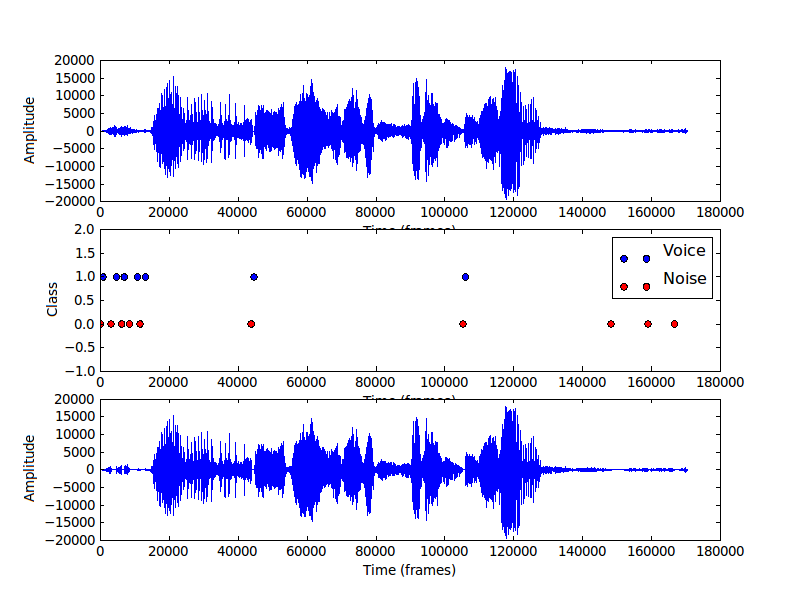
\includegraphics[width=10cm]{ultimation.png}
    \caption{Classification diagram for unseen data from a seen speaker}
\end{figure}

This shows us that firstly, we have built a system that is relatively robust to
speakers that it has been seen before, regardless of the fact that we haven't
seen the specific speech data before. This is encouraging because it indicates
that this system will work in future cases where the speaker has been seen
before.  More importantly this indicates that the classifier has a very high
level of sensitivity as it accurately classified the two pauses within the
overall speech.

A possible problem that is brought up by this is that very quiet utterances
flick back and forth between the background noise and speech class: this could
be annoying if it repeatedly happens and brings to bear the idea of a smoothing
system/long term classifier that uses more information from the long term
context of speech instead of only the short term context which is what the
classifier system that we have built provides.

\section{Use of different classification algorithms}

The choice to use the Random Forest classification algorithm was very much a
decision made based on the author's experience, and in this section we aim to
see whether any of the other classification techniques mentioned in the
technical background section prove to give a better classification rate on the
data set. Whilst the features were very much generated with a random forest in
mind, in the implementation chapter, we showed that the features themselves
give relatively independant views on the data set, with low correlation between
most of the features.

With this in mind, we decided to use all of the ensemble methods discussed
earlier, a simple decision tree algorithm and the k nearest neighbor method.
These represent a broad stroke of classification algorithms used today and will
hopefully reveal as to whether or not our decision to use the Random Forest
classifier was a correct one. For all classifiers we have reported the ROC
curves in \ref{fig:multiclass-roc}, the confusion matrices in
\ref{fig:multiclass-confusion} and the training and test times in
\ref{fig:multiclass-speed}. This experiment was performed by training the
classifiers on half of the data that we have available and using the other half
as unseen testing examples.

\begin{figure}
    \label{fig:multiclass-roc}
    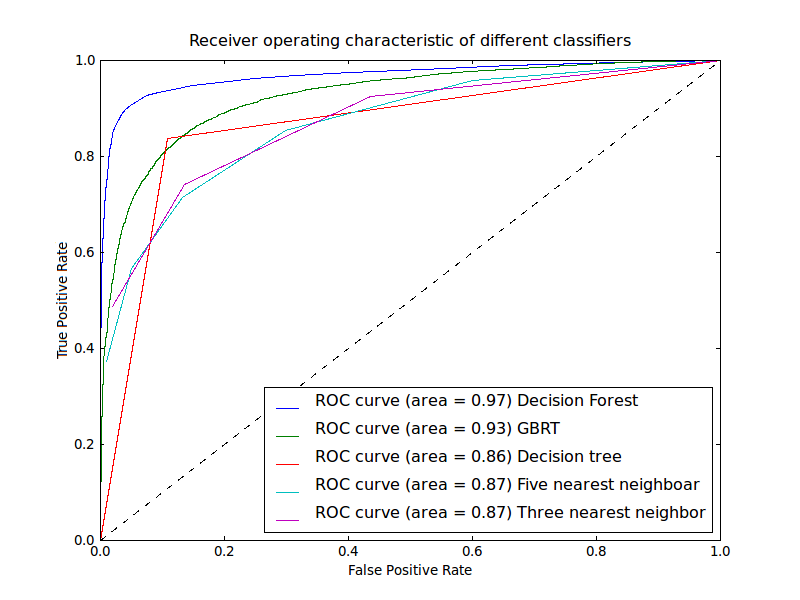
\includegraphics[width=10cm]{roc_different.png}
    \caption{ROC curves of different classifiers}
\end{figure}

\begin{figure}
    \label{fig:multiclass-confusion}

    \begin{tabular}{|l||l|l|}
        \hline
        Random Forest      & Actually Positive & Actually Negative \\ \hline
        Predicted Positive & 9712              & 288               \\ \hline
        Predicted Negative & 1244              & 8756              \\ \hline
    \end{tabular}

    \vspace{0.75cm}

    \begin{tabular}{|l||l|l|}
        \hline
        GBRT               & Actually Positive & Actually Negative \\ \hline
        Predicted Positive & 9209              & 791               \\ \hline
        Predicted Negative & 2291              & 7709              \\ \hline
    \end{tabular}

    \vspace{0.75cm}

    \begin{tabular}{|l||l|l|}
        \hline
        Decision tree      & Actually Positive & Actually Negative \\ \hline
        Predicted Positive & 8912              & 1088               \\ \hline
        Predicted Negative & 1633              & 8367              \\ \hline
    \end{tabular}

    \vspace{0.75cm}

    \begin{tabular}{|l||l|l|}
        \hline
        Five Nearest Neighbor & Actually Positive & Actually Negative \\ \hline
        Predicted Positive    & 8684              & 1316               \\ \hline
        Predicted Negative    & 2861              & 7139              \\ \hline
    \end{tabular}

    \vspace{0.75cm}

    \begin{tabular}{|l||l|l|}
        \hline
        Three Nearest Neighbor & Actually Positive & Actually Negative \\ \hline
        Predicted Positive     & 8642              & 1358               \\ \hline
        Predicted Negative     & 2590              & 7410              \\ \hline
    \end{tabular}

    \vspace{0.75cm}

    \caption{Confusion matrices for different classifiers}

\end{figure}

The reason this experiment is important is that if we can acheive a better
classification accuracy, or classification performance in time/memory with any
of these systems, then it is worth noting. The first thing we note is that the
Random Forest (Decision Forest) gives the best classification rate by some
measure, followed by the Gradient Boosted regression tree algorithm. This does
not contravene expectations as these methods both use a large ensemble of
classifiers (specifically 100 trees were trained for both).

What is more interesting is perhaps that the decision tree classifier acheives
a higher raw classification accuracy than all the algorithms but the decision
forest but has a lower area under the ROC curve. This is because the classifier
implementation that we used for the Decision Tree does not provide output
probabilites but rather a ${0,1}$ discrete classifiation. This means that it's
potentially more accurate classification suffers under the ROC curve metric
because it must be linearly interpolated to the (0,0) and (1,1) points from
it's actual classification output. By comparison we can see that this metric
favours the lower accuracy five nearest and three nearest neighbor classifiers
because they return continuous predictions instead of discrete output and
therefore give are given a more favourable result in the ROC AUC metric.

However, if we look at the confusion matrices of these 4 classifiers we can see
that that the decision tree actually gives a much better overall classification
rate than the five nearest neighbor. These are all important factors to
consider when considering which implementation to use. For example the GBRT
implementation classifes about twice as fast as the random forest
implementation (0.47 seconds versus 0.26 seconds), but has a somewhat lower
accuracy.

From this we can, however, immediately discard the 3 nearest and 5 nearest
neighbor classifiers, they take both the longest to classify (18 seconds
respectively for 320 seconds of audio) and give the lowest training accuracy.
Whilst 18 seconds for 320 may seem like a reasonable time, we envisage this
system sitting in amongst many other components of a VOIP stack, and
introducing any latency may have an impact on user experience, and certainly
the more latent any particular component is, the more optimised the other
components have to be.

All three tree implementations run in under a second with the decision tree
algorithm running in 0.12 seconds, the GBRT running in 0.26 and the Random
forest running in 0.47 seconds. All of these implementations have a very high
classification rate and classification speed and any of them could be used for
a real time system. The result of the Random  Forest running more slowly than
the GBRT is somewhat counterintuitive because our Random Forest runs in
parallel, it performed more slowly in both multithreaded and non-multithreaded
modes, so we assume that something about the reudction of the classifier voting
takes longer than pushing an example through the decision chain in the GBRT.
The authors' recommendation would be to use the decision forest implementation
because it is both the most accurate overall, and in the far left of the ROC
curve (most lax, fewest false negatives).

%\noindent
%This chapter is intended to evaluate what you did.  The content is highly 
%topic-specific, but for many projects will have flavours of the following:
%
%\begin{enumerate}
%\item functional testing, inc. analysis of failure cases,
%\item performance results, and analysis of said results that draw some 
%      form of conclusion,
%      and
%\item evaluation of options and decisions within the project, and/or a
%      comparison with alternatives.
%\end{enumerate}
%
%\noindent
%This chapter often acts to differentiate project quality: even if the work
%completed is of a high technical quality, critical yet objective evaluation 
%and comparison of the outcomes is crucial.  In essence, the reader wants to
%learn something, so the worst examples amount to simple statements of fact 
%(e.g., ``graph X shows the result is Y''); the best examples are analytical 
%and exploratory (e.g., ``graph X shows the result is Y, which means Z; this 
%contradicts [1], which may be because I use a different assumption'').  As 
%such, both positive {\em and} negative outcomes are valid {\em if} presented 
%in a suitable manner.

% -----------------------------------------------------------------------------

\chapter{Conclusion}
\label{chap:conclusion}

{\bf A compulsory chapter, of roughly $2$ pages} 
\vspace{1cm} 

\noindent
The concluding chapter of a thesis is often underutilised, in part because
it is often left until close to the deadline and hence does not get enough 
attention.  Ideally, the chapter will consist of three parts:

\begin{enumerate}
\item (Re)summarise the main contributions and achievements, in essence
      summing up the content.
\item Clearly state the current project status (e.g., ``X is working, Y 
      is not'') and evaluate what has been achieved with respect to the 
      initial aims and objectives (e.g., ``I completed aim X outlined 
      previously, the evidence for this is within Chapter Y'').  There 
      is no problem including aims which were not completed, but it is 
      important to evaluate and/or justify why this is the case.
\item Outline any open problems or future plans.  Rather than treat this
      only as an exercise in what you {\em could} have done given more 
      time, try to focus on any unexplored options or interesting outcomes
      (e.g., ``my experiment for X gave counter-intuitive results, this 
      could be because Y and would form an interesting area for further 
      study'').
\end{enumerate}

% =============================================================================

% Finally, after the main matter, the back matter is specified.  This is
% typically populated with just the bibliography.  LaTeX deals with these
% in one of two ways, namely
%
% - inline, which roughly means the author specifies entries using the 
%   \bibitem macro and typesets them manually, or
% - using BiBTeX, which means entries are contained in a separate file
%   (which is essentially a databased) then inported; this is the 
%   approach used below, with the databased being thesis.bib.
%
% Either way, the each entry has a key (or identifier) which can be used
% in the main matter to cite it, e.g., \cite{X}, \cite[Chapter 2}{Y}.

\backmatter

\bibliography{thesis}

% -----------------------------------------------------------------------------

% The thesis concludes with a set of (optional) appendicies; these are the
% same as chapters in a sense, but once signaled as being appendicies via
% the associated macro, LaTeX manages them appropriatly.

\appendix

\chapter{An Example Appendix}
\label{appx:example}

Content which is not central to, but may enhance the thesis can be
included in one or more appendices; examples include, but are not 
limited to

\begin{itemize}
\item lengthy mathematical proofs, numerical or graphical results
      which are summarised in the main body,
\item sample or example calculations, 
      and
\item results of user studies or questionnaires.
\end{itemize}

\noindent
Note that in line with most research conferences, the marking panel 
is not obliged to read such appendices.

% =============================================================================

\end{document}
